%File: anonymous-submission-latex-2026.tex
\documentclass[letterpaper]{article} % DO NOT CHANGE THIS
\usepackage[submission]{aaai2026}  % DO NOT CHANGE THIS
\usepackage{times}  % DO NOT CHANGE THIS
\usepackage{helvet}  % DO NOT CHANGE THIS
\usepackage{courier}  % DO NOT CHANGE THIS
\usepackage[hyphens]{url}  % DO NOT CHANGE THIS
\usepackage{graphicx} % DO NOT CHANGE THIS
\urlstyle{rm} % DO NOT CHANGE THIS
\def\UrlFont{\rm}  % DO NOT CHANGE THIS
\usepackage{natbib}  % DO NOT CHANGE THIS AND DO NOT ADD ANY OPTIONS TO IT
\usepackage{caption} % DO NOT CHANGE THIS AND DO NOT ADD ANY OPTIONS TO IT
\frenchspacing  % DO NOT CHANGE THIS
\setlength{\pdfpagewidth}{8.5in} % DO NOT CHANGE THIS
\setlength{\pdfpageheight}{11in} % DO NOT CHANGE THIS
%
% These are recommended to typeset algorithms but not required. See the subsubsection on algorithms. Remove them if you don't have algorithms in your paper.
\usepackage{algorithm}
\usepackage{algorithmic}

%
% These are are recommended to typeset listings but not required. See the subsubsection on listing. Remove this block if you don't have listings in your paper.
\usepackage{newfloat}
\usepackage{listings}
\DeclareCaptionStyle{ruled}{labelfont=normalfont,labelsep=colon,strut=off} % DO NOT CHANGE THIS
\lstset{%
	basicstyle={\footnotesize\ttfamily},% footnotesize acceptable for monospace
	numbers=left,numberstyle=\footnotesize,xleftmargin=2em,% show line numbers, remove this entire line if you don't want the numbers.
	aboveskip=0pt,belowskip=0pt,%
	showstringspaces=false,tabsize=2,breaklines=true}
\floatstyle{ruled}
\newfloat{listing}{tb}{lst}{}
\floatname{listing}{Listing}
%
% Keep the \pdfinfo as shown here. There's no need
% for you to add the /Title and /Author tags.
\pdfinfo{
/TemplateVersion (2026.1)
}

% DISALLOWED PACKAGES
% \usepackage{authblk} -- This package is specifically forbidden
% \usepackage{balance} -- This package is specifically forbidden
% \usepackage{color (if used in text)
% \usepackage{CJK} -- This package is specifically forbidden
% \usepackage{float} -- This package is specifically forbidden
% \usepackage{flushend} -- This package is specifically forbidden
% \usepackage{fontenc} -- This package is specifically forbidden
% \usepackage{fullpage} -- This package is specifically forbidden
% \usepackage{geometry} -- This package is specifically forbidden
% \usepackage{grffile} -- This package is specifically forbidden
% \usepackage{hyperref} -- This package is specifically forbidden
% \usepackage{navigator} -- This package is specifically forbidden
% (or any other package that embeds links such as navigator or hyperref)
% \indentfirst} -- This package is specifically forbidden
% \layout} -- This package is specifically forbidden
% \multicol} -- This package is specifically forbidden
% \nameref} -- This package is specifically forbidden
% \usepackage{savetrees} -- This package is specifically forbidden
% \usepackage{setspace} -- This package is specifically forbidden
% \usepackage{stfloats} -- This package is specifically forbidden
% \usepackage{tabu} -- This package is specifically forbidden
% \usepackage{titlesec} -- This package is specifically forbidden
% \usepackage{tocbibind} -- This package is specifically forbidden
% \usepackage{ulem} -- This package is specifically forbidden
% \usepackage{wrapfig} -- This package is specifically forbidden
% DISALLOWED COMMANDS
% \nocopyright -- Your paper will not be published if you use this command
% \addtolength -- This command may not be used
% \balance -- This command may not be used
% \baselinestretch -- Your paper will not be published if you use this command
% \clearpage -- No page breaks of any kind may be used for the final version of your paper
% \columnsep -- This command may not be used
% \newpage -- No page breaks of any kind may be used for the final version of your paper
% \pagebreak -- No page breaks of any kind may be used for the final version of your paperr
% \pagestyle -- This command may not be used
% \tiny -- This is not an acceptable font size.
% \vspace{- -- No negative value may be used in proximity of a caption, figure, table, section, subsection, subsubsection, or reference
% \vskip{- -- No negative value may be used to alter spacing above or below a caption, figure, table, section, subsection, subsubsection, or reference

\setcounter{secnumdepth}{0} %May be changed to 1 or 2 if section numbers are desired.

% The file aaai2026.sty is the style file for AAAI Press
% proceedings, working notes, and technical reports.
%

% Title

% Your title must be in mixed case, not sentence case.
% That means all verbs (including short verbs like be, is, using,and go),
% nouns, adverbs, adjectives should be capitalized, including both words in hyphenated terms, while
% articles, conjunctions, and prepositions are lower case unless they
% directly follow a colon or long dash

% LAMP-Merge：面向单次异步临床模型的长尾感知医学原型融合。
\title{LAMP-Merge: Long-tail-Aware Medical Prototype Merging for One-shot Asynchronous Clinical Models}
\author{
    %Authors
    % All authors must be in the same font size and format.
    Written by AAAI Press Staff\textsuperscript{\rm 1}\thanks{With help from the AAAI Publications Committee.}\\
    AAAI Style Contributions by Pater Patel Schneider,
    Sunil Issar,\\
    J. Scott Penberthy,
    George Ferguson,
    Hans Guesgen,
    Francisco Cruz\equalcontrib,
    Marc Pujol-Gonzalez\equalcontrib
}
\affiliations{
    %Afiliations
    \textsuperscript{\rm 1}Association for the Advancement of Artificial Intelligence\\
    % If you have multiple authors and multiple affiliations
    % use superscripts in text and roman font to identify them.
    % For example,

    % Sunil Issar\textsuperscript{\rm 2},
    % J. Scott Penberthy\textsuperscript{\rm 3},
    % George Ferguson\textsuperscript{\rm 4},
    % Hans Guesgen\textsuperscript{\rm 5}
    % Note that the comma should be placed after the superscript

    1101 Pennsylvania Ave, NW Suite 300\\
    Washington, DC 20004 USA\\
    % email address must be in roman text type, not monospace or sans serif
    proceedings-questions@aaai.org
%
% See more examples next
}

%Example, Single Author, ->> remove \iffalse,\fi and place them surrounding AAAI title to use it
\iffalse
\title{My Publication Title --- Single Author}
\author {
    Author Name
}
\affiliations{
    Affiliation\\
    Affiliation Line 2\\
    name@example.com
}
\fi

\iffalse
%Example, Multiple Authors, ->> remove \iffalse,\fi and place them surrounding AAAI title to use it
\title{My Publication Title --- Multiple Authors}
\author {
    % Authors
    First Author Name\textsuperscript{\rm 1},
    Second Author Name\textsuperscript{\rm 2},
    Third Author Name\textsuperscript{\rm 1}
}
\affiliations {
    % Affiliations
    \textsuperscript{\rm 1}Affiliation 1\\
    \textsuperscript{\rm 2}Affiliation 2\\
    firstAuthor@affiliation1.com, secondAuthor@affilation2.com, thirdAuthor@affiliation1.com
}
\fi


% REMOVE THIS: bibentry
% This is only needed to show inline citations in the guidelines document. You should not need it and can safely delete it.
\usepackage{bibentry}
% END REMOVE bibentry

\begin{document}

\maketitle

\begin{abstract}
%
% 多中心医学模型通常在具有不同设备、不同患者群体和不同诊断标签覆盖范围的医院之间异步训练。本文研究单次异步医学模型融合问题：每个客户端在本地训练后只上传一次，服务器在不访问原始医学图像且不进行联邦优化轮次的条件下构建全局模型。我们将聚合诱导的预测坍缩识别为通用后置融合方法的核心失效模式。研究进一步表明，由于长尾医学先验会使多数类坍缩在准确率上呈现出具有迷惑性的竞争力，原始准确率可能掩盖这一失效。为此，我们提出 LAMP-Merge，即一种长尾感知的医学原型融合框架，它根据客户端侧类别统计重建诊断原型头，并用有界先验偏置校准长尾患病率。在五个医学数据集、五类模型、三种客户端数量和三种非独立同分布偏斜水平上，LAMP-Merge 在 75 个客户端平均单元中的 68 个单元达到或并列超过最强非 LAMP 基线，同时提升了平衡准确率、宏 F1 和预测坍缩诊断指标。
Multicenter medical models are typically trained asynchronously across hospitals with heterogeneous acquisition devices, patient populations, and diagnostic-label coverage. We study single-shot asynchronous medical model merging, where each client uploads its locally trained model only once and the server constructs a global model without accessing raw medical images or conducting federated optimization rounds. We identify aggregation-induced prediction collapse as the central failure mode of general-purpose post-hoc merging methods. Furthermore, we show that long-tailed medical priors can make majority-class collapse deceptively competitive in terms of raw accuracy, thereby masking this failure. To address this issue, we propose LAMP-Merge, a long-tail-aware medical prototype-merging framework that reconstructs a diagnostic prototype head from client-side class statistics and calibrates long-tail prevalence using a bounded prior bias. Across five medical datasets, five model families, three client-population sizes, and three levels of non-IID skew, LAMP-Merge matches or surpasses the strongest non-LAMP baseline in 68 of 75 client-averaged settings, while improving balanced accuracy, macro-F1, and prediction-collapse diagnostic metrics.

%医学模型融合 异步融合 预测性坍缩 长尾校准 隐私保护学习
Index Terms:medical model merging, asynchronous fusion, predictive collapse, long-tail calibration, privacy-preserving learning
\end{abstract}


% Uncomment the following to link to your code, datasets, an extended version or similar.
% You must keep this block between (not within) the abstract and the main body of the paper.
% \begin{links}
%     \link{Code}{https://aaai.org/example/code}
%     \link{Datasets}{https://aaai.org/example/datasets}
%     \link{Extended version}{https://aaai.org/example/extended-version}
% \end{links}

\section{I Introduction}

% 医学人工智能正在从单中心模型开发走向多中心协作部署。临床诊断模型的可靠性通常依赖于跨医院、跨设备和跨患者群体的经验，因为单一机构很难同时覆盖完整疾病谱、罕见病例和不同成像条件。然而，医学数据受到伦理审批、隐私法规、设备差异和院内流程的共同限制，原始影像很难被集中到统一服务器。更现实的协作形态是：各医院在本地完成模型训练，并在训练完成后以有限的信息共享方式参与全局模型构建。
Medical artificial intelligence is transitioning from single-center model development toward multicenter collaborative deployment. The reliability of clinical diagnostic models typically depends on experience spanning hospitals, imaging devices, and patient populations, as no single institution can readily cover the full disease spectrum, rare cases, and diverse imaging conditions simultaneously. However, medical data are jointly constrained by ethical approval requirements, privacy regulations, device heterogeneity, and institutional workflows, making centralization of raw images on a common server difficult. A more practical collaboration paradigm is for hospitals to train models locally and, upon completion, participate in global model construction through limited information sharing.

% 这一现实背景产生了一个单次异步的模型融合需求。不同医院不一定同时在线，也不一定有条件在全局模型更新后反复重新训练；某些中心可能更早完成训练，某些中心可能只在固定窗口内上传模型。与此同时，服务器在部署阶段需要得到一个可供统一使用的全局诊断模型，而不是多个彼此独立、覆盖范围有限的本地模型。因此，本文研究一种事后融合场景：每个客户端只上传一次，服务器在不侵犯患者隐私(不读取客户端原始医学图像)的条件下合成一个共享检查点。
This practical setting motivates a need for single-shot asynchronous model merging. Hospitals may not be online simultaneously or be able to repeatedly retrain after each global-model update; some centers may finish training earlier, whereas others may upload their models only within fixed time windows. Meanwhile, at deployment time, the server must produce a globally usable diagnostic model rather than a collection of independent local models with limited coverage. Accordingly, we study a post-hoc merging setting in which each client uploads exactly once and the server synthesizes a shared checkpoint without compromising patient privacy, i.e., without accessing clients’ raw medical images.
% 医学图像使这一问题具有特殊难度。医院之间的差异不仅表现为图像风格或设备域偏移，还表现为诊断类别可及性的差异：一个中心可能积累了某些常见病或常规检查的大量样本，却几乎没有某些罕见诊断；另一个中心可能具有相反的病例结构。由此得到的本地模型并不是完整全局任务的独立副本，而是带有局部诊断证据的部分专家。更重要的是，医学类别分布通常呈长尾结构，多数类诊断可能占据大量样本，而少数类诊断仍然具有临床意义。一个有效的融合方法必须同时保留分散在不同客户端中的类别证据，并避免把真实长尾患病率误解释为无意义噪声。
Medical imaging makes this problem particularly challenging. Inter-hospital heterogeneity arises not only from image-style and device-domain shifts, but also from differences in diagnostic-class availability: one center may accumulate abundant samples for common diseases or routine examinations while having virtually no cases of certain rare diagnoses, whereas another may exhibit the opposite case composition. The resulting local models are therefore not independent replicas of a complete global task; rather, they are partial experts containing localized diagnostic evidence. More importantly, medical class distributions are typically long-tailed: majority diagnoses may account for a substantial fraction of samples, whereas minority diagnoses remain clinically meaningful. An effective merging method must both preserve class-specific evidence distributed across clients and avoid misinterpreting genuine long-tail prevalence as irrelevant noise.

\begin{figure}[t]
    \centering
    
\includegraphics[width=\linewidth]{figures/intro.png}
    \caption{In multicenter healthcare settings, individual clients typically observe only a subset of the global diagnostic space. Conventional parameter-level model-merging methods can therefore cause the merged global model’s predictions to concentrate on a small number of dominant classes.}
    \label{fig:placeholder}
\end{figure}
% 本文提出 LAMP-Merge，即长尾感知医学原型融合框架。其核心思想是将医学模型融合从全局参数平均问题转化为类别级诊断证据重建问题。客户端在本地使用共享参考特征提取器计算每个诊断类别的聚合原型和类别计数，并仅上传这些类别级统计及本地检查点接口。服务器随后在共享参考空间中构建全局诊断原型分类器，并在类别患病率呈现强长尾结构时引入有界的先验校准。整个过程保持单次上传，不要求服务器访问原始图像、逐样本特征、逐样本 logits 或逐样本预测。
We propose LAMP-Merge, a long-tail-aware medical prototype-merging framework. Its central idea is to recast medical model merging from a problem of global parameter averaging into one of class-level diagnostic-evidence reconstruction. Using a shared reference feature extractor, each client computes an aggregated prototype and sample count for every diagnostic class locally, and uploads only these class-level statistics together with an interface to its local checkpoint. The server then constructs a global diagnostic prototype classifier in the shared reference space and introduces bounded prior calibration when class prevalence exhibits a pronounced long-tailed structure. The entire procedure requires only a single upload and does not require the server to access raw images, per-sample features, per-sample logits, or per-sample predictions.

% 本文贡献总结如下。第一，我们提出并形式化了单次异步医学图像模型融合问题，其中客户端在本地独立训练，服务器只能使用一次上传的信息构建全局模型。第二，我们从医学诊断类别可及性和长尾患病率出发，刻画了该问题区别于一般模型融合任务的核心结构。第三，我们提出 LAMP-Merge，通过客户端侧类别原型和患病率统计重建全局诊断分类器，在保护原始图像隐私的同时缓解融合后的预测坍缩。我们在多个医学影像数据集上开展了大量实验。结果表明，无论原始数据分布情况如何，我们的LAMP-Merge均显著优于所有对比方法。此外，我们的融合方法在训练过程中无需辅助数据集或计算资源支持。
Our main contributions are as follows:
\begin{itemize}
    \item We introduce and formalize the problem of single-shot asynchronous medical image model merging, in which clients train independently on local data and the server must construct a global model using information from a single upload. 
    \item We characterize the key structures that distinguish this setting from general model-merging tasks, namely heterogeneous diagnostic-class availability across medical institutions and long-tailed disease prevalence. \item We propose LAMP-Merge, which reconstructs a global diagnostic classifier from client-side class prototypes and prevalence statistics, mitigating post-merging prediction collapse while preserving the privacy of raw medical images. 
\end{itemize}

We conduct extensive experiments on multiple medical imaging datasets. The results show that LAMP-Merge consistently and substantially outperforms all competing methods across the considered data distributions. Moreover, our merging approach requires neither an auxiliary dataset nor additional computational resources during training.

\section{II Related Works}

\subsection{A. Generic Post-hoc Model Merging}

% 通用事后模型融合旨在整合已经训练完成的模型检查点， 从而避免联合训练或重新训练带来的成本。现有方法可以按照融合变量进行归类。第一类方法直接在权重空间中插值，例如权重平均和 Model Soups；当多个模型仍处在兼容的参数盆地中时，这类方法能够取得较好的融合效果。第二类方法在参数增量空间中运算，例如 Task Arithmetic 将微调模型表示为相对于共享初始化模型的参数位移，并对这些位移进行线性组合。第三类方法试图在平均前消除参数干扰，例如 Git Re-Basin 通过神经元置换对齐减少排列不一致，TIES-Merging 和 DARE 系列方法通过裁剪微小更新、符号投票或随机丢弃并重缩放任务向量来缓解更新冲突。第四类方法进一步引入几何、曲率或鲁棒统计假设，例如 Fisher 融合、RegMean、Model Stock、Breadcrumbs、Iso-C、FreeMerge 和 RobustMerge。
General post-hoc model merging aims to integrate already trained model checkpoints, thereby avoiding the costs of joint training or retraining. Existing methods can be categorized by their merging variables. The first category directly interpolates in weight space, including weight averaging and Model Soups; these methods can merge effectively when models remain in compatible parameter basins. The second category operates in parameter-delta space. For example, Task Arithmetic represents a fine-tuned model as a parameter displacement relative to a shared initialization and linearly combines such displacements. The third category seeks to remove parameter interference before averaging. Git Re-Basin reduces permutation mismatch through neuron-permutation alignment, whereas TIES-Merging and the DARE family mitigate update conflicts by pruning small updates, applying sign voting, or randomly dropping and rescaling task-vector components. The fourth category further incorporates assumptions based on geometry, curvature, or robust statistics, including Fisher merging, RegMean, Model Stock, Breadcrumbs, Iso-C, FreeMerge, and RobustMerge.

% 这些方法构成本文的重要基线，但其融合变量并未针对医学诊断类别建模。它们操作的是全局参数、任务向量、曲率估计、置换结构或更新符号，而不是“客户端 (i) 是否在诊断类别 (c) 上拥有可靠证据”。在多中心医学图像任务中，客户端训练集通常同时存在类别缺失和长尾分布；因此，真正见到某个特定类别的客户端判断的可靠方向会与其他客户端因没见过而缺失或冲突的方向混合。结果是融合模型可能保留多数类方向，同时抑制罕见类或局部缺失类，形成预测分布高度集中的全局坍缩模型。
These methods constitute important baselines in this work, but their merging variables do not model medical diagnostic classes explicitly. They operate on global parameters, task vectors, curvature estimates, permutation structures, or update signs, rather than addressing whether client i possesses reliable evidence for diagnostic class c. In multicenter medical imaging tasks, local client datasets commonly exhibit both missing classes and long-tailed distributions. Consequently, reliable class-specific directions from clients that have observed a particular class are mixed with absent or conflicting directions from clients that have not. The merged model may therefore preserve majority-class directions while suppressing rare or locally absent classes, yielding a globally collapsed model with a highly concentrated predictive distribution.


\subsection{B. Medical Model Merging}

% 医学融合方法通常利用临床数据特有的结构。例如，mTAN 针对非规则采样时间序列使用连续时间注意力，Raindrop 使用图结构建模生理传感器之间的关系，MedFuse 融合胸部 X 光图像与临床时间序列。这些工作表明，医学数据并非通用融合算法的简单应用场景；医学数据具有非规则时间结构、模态异质性、临床测量机制和疾病患病率分布。
Medical fusion methods typically exploit structures specific to clinical data. For example, mTAN employs continuous-time attention for irregularly sampled time series, Raindrop uses graph structures to model relationships among physiological sensors, and MedFuse integrates chest X-ray images with clinical time series. These studies demonstrate that medical data are not merely a straightforward application domain for general-purpose fusion algorithms; they exhibit irregular temporal structures, modality heterogeneity, clinical measurement processes, and disease-prevalence distributions.

% 然而，这些医学融合方法通常融合患者级输入模态或临床表征，而不是融合独立训练得到的医学图像分类器检查点。它们的训练过程往往需要访问患者级样本、时间戳、多模态记录、电子健康记录或服务器端验证反馈。当服务器不能查看客户端原始医学图像、逐样本特征、逐样本 logits 或逐样本预测时，这些方法无法直接用于本文研究的单次模型融合设定。不泄露原始图像的医学模型融合算法也经常依赖验证数据或迭代选择过程，这与我们的单次上传协议相冲突。近期 IEEE TRPMS 的 MedMerge 框架是医学视觉语言模型知识迁移中的重要相关工作，但其目标是不同的跨模态适配场景，而不是同一任务下的异步检查点融合。LAMP-Merge 则将医学结构限制为可上传的类别级统计：客户端在本地计算诊断类别原型和患病率计数，服务器仅根据这些聚合统计构建模型。
However, these medical fusion methods typically combine patient-level input modalities or clinical representations rather than independently trained medical image-classifier checkpoints. Their training procedures often require access to patient-level samples, timestamps, multimodal records, electronic health records, or server-side validation feedback. When the server cannot access clients’ raw medical images, per-sample features, per-sample logits, or per-sample predictions, these methods cannot be directly applied to the single-shot model-merging setting studied here. Medical model-merging methods that avoid disclosing raw images also frequently rely on validation data or iterative selection procedures, which conflicts with our single-upload protocol. The recently proposed MedMerge framework in *IEEE Transactions on Radiation and Plasma Medical Sciences* is an important related work on knowledge transfer for medical vision–language models; however, it targets a different cross-modal adaptation setting rather than asynchronous checkpoint merging for the same task. In contrast, LAMP-Merge restricts medical structure to uploadable class-level statistics: clients compute diagnostic-class prototypes and prevalence counts locally, and the server constructs the model solely from these aggregated statistics.

\subsection{C. Federated and Decentralized Medical Learning}

% 联邦学习和去中心化学习是隐私敏感医学人工智能中的重要方向。FedAvg 及其变体通过多轮通信训练全局模型：服务器发送模型，客户端执行本地优化，然后上传更新供服务器聚合。Swarm Learning 移除了传统中心参数服务器，并使用去中心化协调机制进行多方训练。Gossip Learning 进一步以点对点方式异步传播模型，使参与方通过本地训练和模型交换逐步获得协作收益。
Federated learning and decentralized learning are important paradigms for privacy-sensitive medical AI. FedAvg and its variants train a global model through multiple communication rounds: the server distributes a model, clients perform local optimization, and the server aggregates the uploaded updates. Swarm Learning removes the conventional central parameter server and employs decentralized coordination for multi-party training. Gossip Learning further propagates models asynchronously in a peer-to-peer manner, allowing participants to gradually benefit from collaboration through local training and model exchange.

% 当客户端能够长时间在线、反复通信并从中间全局模型继续训练时，这些方法是适用的。然而，本文研究的问题不是协作训练，而是在训练完成后的单次异步融合。在真实医学部署中，医院可能在不同时间完成训练，并且可能无法承担重复模型分发、训练和上传协议的成本。因此，在我们的设定中，服务器不会向客户端发送一系列全局模型，客户端也不会在观察到服务器融合结果后继续优化。因此，联邦学习和去中心化学习解决的是多轮训练协议问题，而 LAMP-Merge 解决的是单次后置融合问题。LAMP-Merge 只要求每个客户端在本地训练后一次性上传模型和类别级统计，服务器无需建立多轮反馈回路即可生成统一全局诊断模型。
These methods are appropriate when clients can remain online for extended periods, communicate repeatedly, and continue training from intermediate global models. However, the problem studied here is not collaborative training, but single-shot asynchronous merging after local training has been completed. In real-world medical deployments, hospitals may complete training at different times and may be unable to bear the cost of repeated model distribution, training, and upload protocols. Accordingly, in our setting, the server does not distribute a sequence of global models to clients, and clients do not continue optimization after observing the server’s merged result. Federated and decentralized learning therefore address multi-round training protocols, whereas LAMP-Merge addresses single-shot post-hoc merging. LAMP-Merge requires each client to upload its model and class-level statistics only once after local training, enabling the server to produce a unified global diagnostic model without establishing a multi-round feedback loop.

% 医学图像融合需要显式表示类别级诊断可及性，在不多轮通信的情况下同时保护患者的隐私。LAMP-Merge正是针对这一缺口设计：它利用重建逐类别诊断头的方式，由客户端一次性上传类别原型和类别支持数，并在服务端按类别重建全局诊断原型分类器。
Medical image model merging requires an explicit representation of class-level diagnostic availability while preserving patient privacy without multi-round communication. LAMP-Merge is designed to address this gap: clients upload class prototypes and class-support counts in a single round, and the server reconstructs a global diagnostic prototype classifier on a per-class basis, thereby rebuilding the class-specific diagnostic head.

\section{III Method}
\begin{figure}[t]
    \centering
    
\includegraphics[width=\linewidth]{figures/method.png}
    \caption{Local models from multicenter hospitals typically contain only partial diagnostic knowledge, while raw medical images cannot be centrally shared. LAMP-Merge reconstructs a privacy-friendly global medical classifier through diagnostic prototype reconstruction and long-tail prevalence calibration, without accessing raw data or requiring multi-round federated optimization.}
    \label{fig_method}
\end{figure}
\subsection{A. Motivation and Overall Idea}

% 我们发现，在局部类别覆盖的医学场景中，后置参数融合会将多个非退化的局部预测器转化为全局坍缩预测器。而当最常见诊断类别在分布中占据很大比例时，坍缩预测器可以在缺乏真实多类别诊断能力的情况下取得较高准确率。这解释了为什么某些基线在原始准确率上依旧具有竞争力。一个有效的医学融合方法应当避免丢失罕见类别判别能力，同时在任务确实呈强长尾分布时尊重真实患病率信息。
We find that, in medical settings with partial local class coverage, post-hoc parameter merging can transform multiple non-degenerate local predictors into a globally collapsed predictor. When the most prevalent diagnostic class accounts for a large proportion of the data distribution, such a collapsed predictor can achieve high accuracy despite lacking genuine multiclass diagnostic capability. This explains why some baselines remain competitive in terms of raw accuracy. An effective medical merging method should avoid losing discriminative capability for rare classes while respecting true prevalence information when the task genuinely exhibits a strongly long-tailed distribution.

% 为应对这些挑战，我们提出了MedMerge——一个基于类别级诊断原型重建的长尾感知医学模型融合框架，恢复完整诊断空间中的多类别判别方向，从结构上缓解融合后的单类或少数类预测坍缩。然而，为克服去除类别先验可能损害整体准确率的问题，我们进一步设计了长尾患病率校准模块。利用客户端上传的类别患病率计数估计全局诊断先验。具体而言，LAMP-Merge 包含两个核心组件：（1）一种用于聚合多个本地医学客户端中可靠的类别级知识，并重建不易发生坍缩的全局诊断分类器；（2）一种用于在保持多类别判别能力的同时，保留具有临床意义的多数类先验的策略。该设计实现了更加均衡且有效的诊断知识整合，使模型能够在不进行额外联邦训练、不暴露原始医学数据的条件下完成稳健的单次医学模型融合。
To address these challenges, we propose LAMP-Merge, a long-tail-aware medical model-merging framework based on class-level diagnostic prototype reconstruction. It recovers multiclass discriminative directions over the complete diagnostic space, structurally mitigating post-merging prediction collapse toward a single class or a small subset of classes. However, because removing class priors may impair overall accuracy, we further design a long-tail prevalence calibration module that estimates the global diagnostic prior from client-uploaded class-prevalence counts. Specifically, LAMP-Merge comprises two core components:(1) a mechanism for aggregating reliable class-level knowledge across multiple local medical clients and reconstructing a global diagnostic classifier resistant to prediction collapse; and (2) a strategy for preserving clinically meaningful majority-class priors while maintaining multiclass discriminative capability. This design enables more balanced and effective integration of diagnostic knowledge, allowing robust single-shot medical model merging without additional federated training or exposure of raw medical data.

\subsection{B. Overview}

% LAMP-Merge 的核心框架如图所示，其核心思想是将医学模型融合从全局参数平均问题转化为类别条件诊断证据重建问题，并加以类别先验辅佐。
The core framework of LAMP-Merge is illustrated in figure\ref{fig_method}. Its central idea is to recast medical model merging from global parameter averaging into the reconstruction of class-conditional diagnostic evidence, supplemented by class-prior information.

% 值得注意的是，LAMP-Merge 并不要求服务器读取客户端原始图像，也不依赖服务器端验证集、逐样本特征或逐样本预测。客户端上传的信息仅为类别级统计量，因此该框架保持单次异步通信边界，区别于需要多轮模型下发与本地再训练的联邦学习流程。
Notably, LAMP-Merge neither requires the server to access clients’ raw images nor relies on a server-side validation set, per-sample features, or per-sample predictions. Clients upload only class-level statistics; thus, the framework preserves a single-shot asynchronous communication boundary, distinguishing it from federated learning procedures that require repeated model broadcasts and local retraining.

% 该框架由两个关键组件构成：类别级诊断原型重建模块和长尾患病率校准模块，原型重建模块用于恢复完整全局诊断空间中的多类别判别方向；随后校准模块保留合理的类别先验。
The framework comprises two key components: a class-level diagnostic prototype reconstruction module and a long-tail prevalence calibration module. The prototype reconstruction module restores multiclass discriminative directions across the complete global diagnostic space, after which the calibration module retains appropriate class-prior information.

\subsection{C. Diagnostic Prototype Reconstruction Module}
%假设存在 K 个医学客户端。客户端 i 拥有一个私有标注数据集 D_i={(x,y)}，该数据集来自覆盖 C 个诊断类别的类别偏斜医学分布。令 D_i,c 表示客户端 i 中属于诊断类别 c 的子集。在医学划分中，D_i,c 对许多类别都可能为空。因此，一个客户端可以对一部分诊断可靠，但对未见类别不可靠。类别无关的参数融合没有显式机制来保留这种局部可靠性结构。
Assume $K$ medical clients. Client $i$ owns a private labeled dataset $D_i=\{(x,y)\}$ drawn from a class-skewed medical distribution over $C$ diagnosis classes. Let $D_{i,c}$ denote the subset of client $i$ belonging to diagnosis class $c$. In medical partitions, $D_{i,c}$ can be empty for many classes. Thus, a client can be reliable for a subset of diagnoses but unreliable for unseen classes. A class-agnostic parameter merge has no explicit mechanism to preserve this local reliability structure.


% 因此，LAMP-Merge 首先在共享参考特征空间中重建逐类别诊断头。令 phi_0 表示在本地训练前由共享模型配置实例化得到的冻结参考骨干网络，T(.) 表示评估变换。对于每个诊断类别 c，客户端 i 计算参考空间类别原型 mu_i,c，其中 n_i,c=|D_i,c| 是类别支持数。如果 n_i,c=0，则客户端为该类别上传零支持数，并且不贡献原型证据。
Therefore, LAMP-Merge first reconstructs a class-wise diagnostic head in the shared reference feature space. Let $\phi_0$ be the frozen reference backbone instantiated from the shared model configuration before local training, and let $T(\cdot)$ be the evaluation transform. For each diagnosis class $c$, client $i$ computes a reference-space class prototype
\begin{equation}
\mu_{i,c}=\frac{1}{n_{i,c}}\sum_{(x,y)\in D_i}\mathbf{1}[y=c]\phi_0(T(x)),
\end{equation}
where $n_{i,c}=|D_{i,c}|$ is the class support count. If $n_{i,c}=0$, the client uploads zero support for that class and contributes no prototype evidence.

% 服务器将支持数转换为证据权重，其中 gamma=0.45 为默认证据指数。客户端 i 对类别 c 的归一化可靠性为 alpha_i,c。随后，全局诊断原型 p_c 由各客户端原型按照可靠性加权得到。最后，LAMP-Merge 合成一个余弦原型分类器，其中 s=20 为默认分类头缩放因子。该模块解决了当前算法的痛点：它保留了每个客户端具有证据的类别，并重建全局多类别诊断头。
The server converts support counts into evidence weights:
\begin{equation}
e_{i,c}=(n_{i,c}+1)^\gamma \mathbf{1}[n_{i,c}>0],
\end{equation}
where $\gamma=0.45$ is the default evidence exponent. The normalized reliability of client $i$ for class $c$ is
\begin{equation}
\alpha_{i,c}=\frac{e_{i,c}}{\sum_{j=1}^{K} e_{j,c}}.
\end{equation}
The global diagnosis prototype is then
\begin{equation}
p_c=\sum_{i=1}^{K}\alpha_{i,c}\mu_{i,c}.
\end{equation}
Finally, LAMP-Merge synthesizes a cosine prototype classifier:
\begin{equation}
w_c=s\frac{p_c}{\|p_c\|_2},
\end{equation}
where $s=20$ is the default head scale. This module addresses a key limitation of existing methods: it preserves the classes for which each client has supporting evidence and reconstructs a global multiclass diagnostic head.

\subsection{D. Long-tail Prevalence Calibration}

% 得到这个全新的诊断头之后，为应对真实医学任务包含的长尾患病率，每个客户端还上传类别患病率计数 m_i,c。服务器据此估计全局类别先验 pi_c。我们使用 r=C max_c pi_c 度量主导类别不平衡。该模块仅在 r>tau 时激活，其中 tau=2.5 为默认值。激活后，添加一个中心化的对数先验偏置 b_c，其默认最大校准强度为 lambda=5.0。最终得分为 score_c(x)。该偏置是中心化且有界的，并附着在原型分类器上；它校准患病率，但不替代 M1 重建的多类别诊断方向。
After obtaining this newly reconstructed diagnostic head, each client additionally uploads class-prevalence counts $m_{i,c}$ to account for the long-tailed prevalence inherent in real-world medical tasks. The server estimates the global class prior
\begin{equation}
\pi_c=\frac{\sum_{i=1}^{K}m_{i,c}}{\sum_{k=1}^{C}\sum_{i=1}^{K}m_{i,k}}.
\end{equation}
We measure dominant-class imbalance by
\begin{equation}
r=C\max_c \pi_c.
\end{equation}
The module is activated only when $r>\tau$, where $\tau=2.5$ by default. When activated, it adds a centered log-prior bias
\begin{equation}
b_c=\lambda\left(\log\pi_c-\frac{1}{C}\sum_{k=1}^{C}\log\pi_k\right),
\end{equation}
with default maximum calibration strength $\lambda=5.0$. The final score is
\begin{equation}
\mathrm{score}_c(x)=w_c^\top\phi_0(T(x))+b_c.
\end{equation}
The bias is centered, bounded, and attached to the prototype classifier; it calibrates prevalence without replacing the multi-class diagnostic directions reconstructed by the Diagnostic Prototype Reconstruction Module.

\section{Experiments}

\subsection{A. Experimental Settings}

\subsubsection{1) Base Models and Merging Setup:} 
% 实验遵循单次异步模型融合流程。每个客户端先在自己的医学图像数据上独立训练本地模型，在本地计算 LAMP-Merge 所需的类别级统计，包括类别支持数、参考空间类别原型和类别患病率计数，并与本地检查点接口一起上传一次。随后服务器只根据上传的检查点和类别级统计执行一次后置融合，并在全局测试集上评估融合模型。
Experiments follow a single-shot asynchronous model-merging protocol. Each client first independently trains a local model on its own medical imaging data, then computes the class-level statistics required by LAMP-Merge locally, including class-support counts, reference-space class prototypes, and class-prevalence counts. These statistics are uploaded once together with an interface to the local checkpoint. The server subsequently performs a single post-hoc merging step using only the uploaded checkpoints and class-level statistics, and evaluates the resulting merged model on a global test set.

% 我们评估五类基础模型。标准视觉骨干网络包括 ResNet、ConvNeXt、ViT-Tiny 和 Swin-Tiny；视觉语言骨干网络包括 CLIP-ViT-B/32。对于每个数据集-模型组合，我们构造非独立同分布客户端划分，客户端数量 K 属于 {3,5,7}，Dirichlet 偏斜参数 beta 属于 {0,0.01,0.1}，随机种子固定为 42。客户端平均结果先固定数据集、模型和 K，再对三个 beta 值求平均。
We evaluate five model families. The standard vision backbones include ResNet, ConvNeXt, ViT-Tiny, and Swin-Tiny, and the vision-language backbone is CLIP-ViT-B/32. For each dataset-model pair, we construct non-IID client partitions with $K\in\{3,5,7\}$ clients and Dirichlet skew parameter $\beta\in\{0,0.01,0.1\}$, using seed 42. A client-average result fixes the dataset, model, and $K$, and then averages over the three $\beta$ values.

% 所有实验运行在配备两颗 Intel Xeon Silver 4210 CPU、四张 NVIDIA GeForce RTX 2080 Ti GPU 的服务器上；软件环境为 conda 环境 MM，使用 Python 3.10.20、PyTorch 2.6.0+cu118 和 CUDA runtime 11.8。
All experiments were run on a server with two Intel(R) Xeon(R) Silver 4210 CPUs, four NVIDIA GeForce RTX 2080 Ti GPUs, and the conda environment \texttt{MM} with Python 3.10.20, PyTorch 2.6.0+\texttt{cu118}, and CUDA runtime 11.8.

\subsubsection{2) Evaluation Datasets:}

\begin{table}[t]
\centering
\caption{Dataset statistics used in the experiments.}
\label{tab:dataset-stats}
\scriptsize
\setlength{\tabcolsep}{3.2pt}
\begin{tabular}{lrrrrr}
\hline
Dataset & Classes & Channels & Train & Val & Test \\
\hline
Blood & 8 & 3 & 11959 & 1712 & 3421 \\
Derma & 7 & 3 & 7007 & 1003 & 2005 \\
Organ-C & 11 & 1 & 12975 & 2392 & 8216 \\
Organ-S & 11 & 1 & 13932 & 2452 & 8827 \\
Ultrasound & 8 & 3 & 3869 & 549 & 1113 \\
\hline
Total & -- & -- & 49742 & 8108 & 23582 \\
\hline
\end{tabular}
\end{table}

% \subsubsection{Evaluation Datasets}
% 我们在多个具有代表性的医学图像基准数据集上对融合后的模型进行评估。这些数据集覆盖血液显微图像、皮肤镜图像、腹部 CT 器官切片和超声图像等关键医学影像模态，并包含细胞形态识别、皮肤病变诊断、器官结构识别和超声结构判别等任务。所用数据集包括：
We evaluate the merged models on multiple representative medical image benchmarks. These datasets cover key medical imaging modalities, including blood-cell microscopy, dermoscopy, abdominal CT organ slices, and ultrasound images, and involve cell morphology recognition, skin-lesion diagnosis, organ-structure recognition, and ultrasound-structure discrimination. The datasets used in the experiments include:

\begin{itemize}
\item \textbf{Blood}: an eight-class blood-cell microscopy dataset for hematological morphology classification, focusing on fine-grained cellular appearance and inter-class morphological similarity.
\item \textbf{Derma}: a seven-class dermoscopic skin-lesion dataset, characterized by strong long-tailed prevalence and visually subtle lesion categories.
\item \textbf{Organ-C}: an 11-class abdominal CT dataset in the coronal view, evaluating organ-category recognition under grayscale cross-sectional imaging.
\item \textbf{Organ-S}: an 11-class abdominal CT dataset in the sagittal view, complementing Organ-C with a different anatomical imaging plane.
\item \textbf{Ultrasound}: an eight-class ultrasound image dataset, covering structure recognition under modality-specific speckle noise and low-contrast boundaries.
\end{itemize}

%  这些基准数据集覆盖了医学图像分类任务中的多种成像场景，为评估融合模型的跨模态鲁棒性、类别判别能力和任务泛化能力提供了系统测试平台。我们针对这些数据集开展系统性实验，以分析 LAMP-Merge 在不同医学图像类型和不同类别分布条件下的性能表现。
These benchmark datasets cover diverse imaging settings in medical image classification, providing a systematic testbed for evaluating the cross-modality robustness, class-discriminative capability, and task generalization of merged models. We conduct systematic experiments on these datasets to analyze the performance of LAMP-Merge across different medical image types and class-distribution conditions.


\subsubsection{3) Evaluation Metrics:}
% 主实验仅使用准确率作为模型选择与横向比较指标。给定 N 张测试图像，令 y_n 表示真实标签，hat y_n 表示模型预测标签，则准确率定义为：
The main experiments use only Accuracy (ACC) as the model-selection and cross-method comparison metric. Given $N$ test images, let $y_n$ denote the ground-truth label and $\hat y_n$ denote the predicted label. ACC is defined as
\begin{equation}
\mathrm{ACC}=\frac{1}{N}\sum_{n=1}^{N}\mathbf{1}[\hat y_n=y_n].
\end{equation}

\subsubsection{4) Hyperparameter Settings:}

% 除非另有说明，LAMP-Merge 在所有数据集、骨干网络、客户端数量和偏斜水平上使用同一组超参数：证据指数 gamma=0.45、原型头缩放因子 s=20、长尾激活阈值 tau=2.5，以及患病率校准强度 lambda=5.0。
Unless otherwise stated, LAMP-Merge uses one fixed hyperparameter configuration for all datasets, backbones, client counts, and skew levels: evidence exponent $\gamma=0.45$, prototype head scale $s=20$, long-tail activation threshold $\tau=2.5$, and prevalence calibration strength $\lambda=5.0$. 


\subsection{B. Comparison With the State of the Arts}
% 我们将 LAMP-Merge 与十二种后置融合基线比较，包括 avg、ties、dare_linear、dare_ties、regmean、fisher、breadcrumbs、model_stock、from、iso_c、free_merge 和 robustmerge。这些基线覆盖权重平均、任务向量修剪、符号冲突处理、曲率或均值校正、模型库存和鲁棒融合等当前主流后置模型融合路线。主比较采用客户端平均准确率：对于每个固定的数据集、模型和客户端数量，先对三个 beta 偏斜水平求平均，再比较不同融合方法。若 LAMP-Merge 在某个单元中大于或等于最强非 LAMP 基线，则该单元计为成功。
We compare LAMP-Merge with twelve post-hoc merging baselines: \texttt{avg}, \texttt{ties}, \texttt{dare\_linear}, \texttt{dare\_ties}, \texttt{regmean}, \texttt{fisher}, \texttt{breadcrumbs}, \texttt{model\_stock}, \texttt{from}, \texttt{iso\_c}, \texttt{free\_merge}, and \texttt{robustmerge}. These baselines cover representative routes in current post-hoc model merging, including weight averaging, task-vector trimming, sign-conflict resolution, curvature or mean correction, model stock, and robust merging. The main comparison uses client-average ACC: for each fixed dataset, model, and client number, we first average over the three $\beta$ skew levels and then compare merging methods. A cell is counted as successful when LAMP-Merge is greater than or equal to the strongest non-LAMP baseline in that cell.

% 表 2 至表 6 给出了完整客户端平均结果。在 75 个客户端平均单元中，LAMP-Merge 在 68 个单元达到或并列超过最强非 LAMP 基线，对应 90.7%。该结果表明，LAMP-Merge 的收益不是由单一客户端数量、单一划分偏斜或单一模型族产生的偶然现象，而是在多种医学图像模态和多种骨干网络上稳定出现。
Tables~\ref{tab:client-avg-resnet}--\ref{tab:client-avg-clip} report the full client-average results. Across the 75 client-average cells, LAMP-Merge wins or ties the strongest non-LAMP baseline in 68 cells, corresponding to 90.7\%. This result indicates that the gain is not an accidental effect of one client number, one partition skew, or one model family; instead, it appears consistently across multiple medical image modalities and backbone architectures.


\begin{table*}[t]
\centering
\scriptsize
\setlength{\tabcolsep}{2.6pt}
\caption{Client-average test accuracy on resnet. Each entry averages the three Dirichlet settings for a fixed client number.Best in blod and second with \underline{underline}. These notes are the same to others.}
\label{tab:client-avg-resnet}
\resizebox{\textwidth}{!}{%
\begin{tabular}{lccccccccccccccc}
\hline
& \multicolumn{3}{c}{Blood} & \multicolumn{3}{c}{Derma} & \multicolumn{3}{c}{Organ-C} & \multicolumn{3}{c}{Organ-S} & \multicolumn{3}{c}{Ultrasound} \\
\cline{2-4}\cline{5-7}\cline{8-10}\cline{11-13}\cline{14-16}
Method & $K=3$ & $K=5$ & $K=7$ & $K=3$ & $K=5$ & $K=7$ & $K=3$ & $K=5$ & $K=7$ & $K=3$ & $K=5$ & $K=7$ & $K=3$ & $K=5$ & $K=7$ \\
\hline
\texttt{avg} & 0.3345 & 0.2467 & 0.2822 & 0.6291 & 0.4700 & 0.6244 & 0.2261 & 0.1772 & 0.1396 & \underline{0.2864} & 0.1794 & 0.2475 & 0.2435 & 0.1581 & 0.1542 \\
\texttt{ties} & 0.2601 & 0.1872 & 0.1787 & 0.5995 & 0.4841 & 0.6484 & 0.2650 & 0.1684 & \underline{0.2118} & 0.1981 & 0.1915 & 0.1874 & \underline{0.3477} & 0.1989 & 0.1854 \\
\texttt{dare\_linear} & 0.2832 & \underline{0.2856} & 0.2392 & 0.6357 & 0.4841 & 0.6288 & 0.2018 & \underline{0.2588} & 0.1650 & 0.2545 & 0.2245 & \underline{0.2537} & 0.2162 & 0.1728 & 0.1608 \\
\texttt{dare\_ties} & 0.3194 & 0.1935 & 0.1780 & 0.5375 & 0.4825 & 0.5558 & 0.1851 & 0.1515 & 0.1859 & 0.1790 & 0.1352 & 0.1730 & 0.2932 & 0.1635 & 0.1890 \\
\texttt{regmean} & \underline{0.3460} & 0.2369 & \underline{0.3407} & 0.5812 & 0.2843 & 0.5022 & 0.2405 & 0.1340 & 0.1388 & 0.2504 & 0.1623 & 0.1493 & 0.2276 & 0.1695 & 0.1318 \\
\texttt{fisher} & 0.3196 & 0.2237 & 0.2608 & 0.6707 & \underline{0.6702} & \underline{0.6690} & \underline{0.2973} & 0.1741 & 0.1812 & 0.2010 & \underline{0.2956} & 0.1963 & 0.2333 & 0.1860 & \underline{0.2513} \\
\texttt{breadcrumbs} & 0.0854 & 0.1417 & 0.1460 & 0.0495 & 0.2913 & 0.1721 & 0.0766 & 0.0676 & 0.0685 & 0.0802 & 0.0948 & 0.0603 & 0.1225 & 0.1273 & 0.1021 \\
\texttt{model\_stock} & 0.2420 & 0.1824 & 0.1975 & 0.6216 & 0.4311 & 0.5721 & 0.1225 & 0.1274 & 0.1185 & 0.2742 & 0.1578 & 0.2012 & 0.1791 & 0.1321 & 0.1578 \\
\texttt{from} & 0.2989 & 0.2306 & 0.2052 & \underline{0.6713} & 0.4369 & 0.6580 & 0.2350 & 0.1560 & 0.1520 & 0.2207 & 0.2087 & 0.2476 & 0.2309 & 0.1506 & 0.2063 \\
\texttt{iso\_c} & 0.3278 & 0.2748 & 0.3023 & 0.5049 & 0.4422 & 0.6416 & 0.2331 & 0.1629 & 0.1383 & 0.2736 & 0.2118 & 0.2453 & 0.2615 & 0.1698 & 0.1554 \\
\texttt{free\_merge} & 0.3345 & 0.2467 & 0.2822 & 0.6291 & 0.4700 & 0.6246 & 0.2261 & 0.1771 & 0.1396 & 0.2863 & 0.1793 & 0.2475 & 0.2435 & 0.1581 & 0.1545 \\
\texttt{robustmerge} & 0.3401 & 0.2430 & 0.2256 & 0.2956 & 0.2085 & 0.3942 & 0.2458 & 0.1764 & 0.1653 & 0.2680 & 0.2227 & 0.2301 & 0.2189 & \underline{0.2231} & 0.1707 \\
\textbf{LAMP-Merge} & \textbf{0.8002} & \textbf{0.7999} & \textbf{0.8007} & \textbf{0.6745} & \textbf{0.6761} & \textbf{0.6763} & \textbf{0.6074} & \textbf{0.6069} & \textbf{0.6076} & \textbf{0.5531} & \textbf{0.5524} & \textbf{0.5517} & \textbf{0.4762} & \textbf{0.4762} & \textbf{0.4762} \\
\hline
\end{tabular}
}
\end{table*}

\begin{table*}[t]
\centering
\scriptsize
\setlength{\tabcolsep}{2.6pt}
\caption{Client-average test accuracy on convnext. Each entry averages the three Dirichlet settings for a fixed client number.}
\label{tab:client-avg-convnext}
\resizebox{\textwidth}{!}{%
\begin{tabular}{lccccccccccccccc}
\hline
& \multicolumn{3}{c}{Blood} & \multicolumn{3}{c}{Derma} & \multicolumn{3}{c}{Organ-C} & \multicolumn{3}{c}{Organ-S} & \multicolumn{3}{c}{Ultrasound} \\
\cline{2-4}\cline{5-7}\cline{8-10}\cline{11-13}\cline{14-16}
Method & $K=3$ & $K=5$ & $K=7$ & $K=3$ & $K=5$ & $K=7$ & $K=3$ & $K=5$ & $K=7$ & $K=3$ & $K=5$ & $K=7$ & $K=3$ & $K=5$ & $K=7$ \\
\hline
\texttt{avg} & 0.1565 & 0.1122 & 0.1384 & 0.2966 & \underline{0.4830} & \textbf{0.6688} & 0.1037 & 0.1218 & 0.0944 & 0.1308 & 0.1035 & 0.1416 & 0.1506 & 0.1506 & 0.1252 \\
\texttt{ties} & 0.1715 & 0.1214 & 0.1524 & 0.2966 & 0.1797 & 0.2713 & 0.1217 & 0.0786 & 0.0716 & 0.1123 & 0.0761 & 0.0796 & 0.1518 & 0.1456 & 0.1291 \\
\texttt{dare\_linear} & 0.1756 & 0.1122 & 0.1345 & 0.2705 & \underline{0.4830} & 0.4830 & 0.1035 & 0.0699 & 0.1085 & 0.1282 & 0.1035 & 0.0797 & 0.1575 & 0.1575 & 0.1264 \\
\texttt{dare\_ties} & 0.1096 & 0.1519 & 0.1497 & 0.0908 & 0.2798 & 0.2451 & 0.1305 & 0.1346 & 0.0770 & 0.1096 & 0.0946 & 0.0709 & 0.1456 & 0.1297 & 0.1500 \\
\texttt{regmean} & 0.1565 & 0.0817 & \underline{0.1856} & 0.2633 & 0.0773 & 0.2720 & 0.1143 & 0.1017 & 0.0768 & 0.1014 & 0.1259 & 0.1038 & 0.1575 & 0.1539 & 0.1500 \\
\texttt{fisher} & 0.1565 & 0.0999 & 0.1189 & \underline{0.4825} & 0.2638 & 0.2971 & 0.1003 & 0.0974 & 0.0915 & 0.0604 & 0.0517 & 0.0843 & \underline{0.1695} & 0.1360 & 0.1456 \\
\texttt{breadcrumbs} & 0.1516 & 0.1366 & 0.1163 & 0.0524 & 0.2766 & 0.4630 & 0.1031 & \underline{0.1444} & 0.1574 & 0.1516 & \underline{0.1554} & \underline{0.2077} & 0.1384 & 0.1363 & 0.1363 \\
\texttt{model\_stock} & 0.1756 & 0.1144 & 0.1778 & 0.2966 & \underline{0.4830} & \textbf{0.6688} & 0.1276 & 0.1218 & 0.1385 & 0.1308 & 0.1035 & 0.1935 & 0.1575 & 0.1291 & 0.1479 \\
\texttt{from} & 0.1565 & 0.1083 & 0.1671 & 0.2966 & 0.3406 & 0.4569 & 0.1232 & 0.1224 & 0.0650 & 0.1324 & 0.1105 & 0.0897 & 0.1575 & \underline{0.1578} & 0.1087 \\
\texttt{iso\_c} & \underline{0.1947} & \underline{0.1865} & 0.1480 & 0.2971 & \underline{0.4830} & \textbf{0.6688} & 0.0991 & 0.0699 & 0.0945 & 0.0789 & 0.1477 & 0.0867 & 0.1518 & 0.1291 & 0.1605 \\
\texttt{free\_merge} & 0.1575 & 0.1190 & 0.1384 & 0.2971 & \underline{0.4830} & \textbf{0.6688} & 0.0906 & 0.1218 & 0.1385 & 0.1308 & 0.1035 & 0.1416 & 0.1506 & 0.1291 & \underline{0.1695} \\
\texttt{robustmerge} & 0.1410 & 0.1405 & 0.0752 & 0.0908 & 0.4507 & 0.4830 & \underline{0.1394} & 0.1218 & \underline{0.1793} & \underline{0.2354} & 0.0961 & \underline{0.2077} & 0.1300 & 0.1135 & 0.1363 \\
\textbf{LAMP-Merge} & \textbf{0.8482} & \textbf{0.8483} & \textbf{0.8493} & \textbf{0.5992} & \textbf{0.5920} & \underline{0.5852} & \textbf{0.6482} & \textbf{0.6480} & \textbf{0.6495} & \textbf{0.5977} & \textbf{0.5985} & \textbf{0.5990} & \textbf{0.4259} & \textbf{0.4259} & \textbf{0.4259} \\
\hline
\end{tabular}
}
\end{table*}

\begin{table*}[t]
\centering
\scriptsize
\setlength{\tabcolsep}{2.6pt}
\caption{Client-average test accuracy on vit\_t. Each entry averages the three Dirichlet settings for a fixed client number.}
\label{tab:client-avg-vit-t}
\resizebox{\textwidth}{!}{%
\begin{tabular}{lccccccccccccccc}
\hline
& \multicolumn{3}{c}{Blood} & \multicolumn{3}{c}{Derma} & \multicolumn{3}{c}{Organ-C} & \multicolumn{3}{c}{Organ-S} & \multicolumn{3}{c}{Ultrasound} \\
\cline{2-4}\cline{5-7}\cline{8-10}\cline{11-13}\cline{14-16}
Method & $K=3$ & $K=5$ & $K=7$ & $K=3$ & $K=5$ & $K=7$ & $K=3$ & $K=5$ & $K=7$ & $K=3$ & $K=5$ & $K=7$ & $K=3$ & $K=5$ & $K=7$ \\
\hline
\texttt{avg} & 0.1343 & 0.1082 & 0.1160 & 0.4638 & 0.4369 & 0.3696 & 0.1657 & 0.1043 & 0.0952 & 0.0844 & 0.0852 & 0.1710 & 0.1450 & 0.1327 & \underline{0.1884} \\
\texttt{ties} & 0.0796 & 0.1421 & 0.1285 & 0.4780 & 0.3498 & 0.4615 & 0.1341 & 0.1223 & 0.0953 & 0.1192 & 0.1002 & 0.1597 & \underline{0.2001} & 0.1306 & 0.1018 \\
\texttt{dare\_linear} & \underline{0.2397} & 0.1129 & 0.1387 & 0.2850 & 0.1002 & 0.1204 & 0.1534 & 0.0946 & 0.0704 & 0.0748 & 0.0549 & 0.1611 & 0.1366 & 0.1051 & 0.1435 \\
\texttt{dare\_ties} & 0.0735 & 0.1189 & 0.1146 & 0.2735 & 0.4502 & 0.3528 & 0.1252 & 0.0903 & 0.1033 & 0.0541 & 0.0874 & 0.0591 & 0.1447 & 0.1120 & 0.1042 \\
\texttt{regmean} & 0.1748 & 0.1417 & 0.1290 & 0.5114 & 0.3667 & \underline{0.6658} & 0.1250 & 0.0964 & 0.0983 & \underline{0.1263} & 0.0717 & 0.1068 & 0.1491 & 0.1384 & 0.1144 \\
\texttt{fisher} & 0.1166 & \underline{0.1512} & \underline{0.1944} & 0.4780 & 0.2042 & 0.4820 & 0.0799 & 0.1072 & 0.1424 & 0.0856 & \underline{0.1218} & 0.1222 & 0.1611 & 0.1315 & 0.1420 \\
\texttt{breadcrumbs} & 0.1363 & 0.1039 & 0.1300 & 0.0489 & 0.2572 & 0.0607 & 0.0773 & 0.1000 & \underline{0.1644} & 0.1237 & 0.0483 & 0.1219 & 0.1360 & 0.1141 & 0.1524 \\
\texttt{model\_stock} & 0.1940 & 0.1120 & 0.1134 & 0.3805 & 0.3079 & 0.2735 & 0.1488 & 0.1227 & 0.1215 & 0.0893 & 0.0859 & \underline{0.1867} & 0.1599 & 0.1809 & 0.1641 \\
\texttt{from} & 0.1802 & 0.0781 & 0.1405 & 0.4695 & \underline{0.5121} & \textbf{0.6688} & \underline{0.2148} & \underline{0.1301} & 0.0972 & 0.0772 & 0.0798 & 0.1485 & 0.1836 & 0.1743 & 0.1776 \\
\texttt{iso\_c} & 0.1234 & 0.1483 & 0.1018 & \underline{0.5709} & 0.4529 & 0.2306 & 0.1084 & 0.0567 & 0.0897 & 0.0611 & 0.0531 & 0.1081 & 0.1417 & 0.1527 & 0.1869 \\
\texttt{free\_merge} & 0.1989 & 0.1457 & 0.1392 & 0.4630 & 0.4770 & 0.3855 & 0.1425 & 0.0980 & 0.0759 & 0.0727 & 0.0914 & 0.1643 & 0.1405 & 0.1593 & 0.1647 \\
\texttt{robustmerge} & 0.1482 & 0.1070 & 0.1425 & 0.0347 & 0.2768 & 0.1724 & 0.0954 & 0.0617 & 0.1438 & 0.1260 & 0.0707 & 0.1217 & 0.1698 & \underline{0.1854} & 0.1563 \\
\textbf{LAMP-Merge} & \textbf{0.8523} & \textbf{0.8522} & \textbf{0.8516} & \textbf{0.5970} & \textbf{0.5938} & 0.5860 & \textbf{0.5805} & \textbf{0.5790} & \textbf{0.5790} & \textbf{0.5406} & \textbf{0.5372} & \textbf{0.5388} & \textbf{0.4645} & \textbf{0.4645} & \textbf{0.4645} \\
\hline
\end{tabular}
}
\end{table*}

\begin{table*}[t]
\centering
\scriptsize
\setlength{\tabcolsep}{2.6pt}
\caption{Client-average test accuracy on swin\_tiny. Each entry averages the three Dirichlet settings for a fixed client number.}
\label{tab:client-avg-swin-tiny}
\resizebox{\textwidth}{!}{%
\begin{tabular}{lccccccccccccccc}
\hline
& \multicolumn{3}{c}{Blood} & \multicolumn{3}{c}{Derma} & \multicolumn{3}{c}{Organ-C} & \multicolumn{3}{c}{Organ-S} & \multicolumn{3}{c}{Ultrasound} \\
\cline{2-4}\cline{5-7}\cline{8-10}\cline{11-13}\cline{14-16}
Method & $K=3$ & $K=5$ & $K=7$ & $K=3$ & $K=5$ & $K=7$ & $K=3$ & $K=5$ & $K=7$ & $K=3$ & $K=5$ & $K=7$ & $K=3$ & $K=5$ & $K=7$ \\
\hline
\texttt{avg} & 0.1565 & 0.1186 & 0.1524 & 0.4569 & \underline{0.4830} & \textbf{0.6688} & 0.1068 & 0.1294 & 0.0787 & 0.0682 & 0.0604 & 0.1381 & 0.1527 & 0.1294 & 0.1465 \\
\texttt{ties} & 0.0972 & 0.1190 & 0.1384 & 0.0841 & 0.0780 & \textbf{0.6688} & 0.1160 & 0.0702 & 0.0934 & 0.0734 & 0.0607 & 0.1107 & 0.1695 & 0.1303 & 0.1261 \\
\texttt{dare\_linear} & 0.1565 & 0.1161 & 0.1825 & 0.4569 & 0.2771 & 0.4630 & 0.1155 & 0.1272 & 0.0776 & 0.0640 & 0.0720 & 0.1381 & 0.1743 & 0.1536 & 0.1497 \\
\texttt{dare\_ties} & 0.1384 & 0.1162 & 0.1384 & 0.2961 & 0.2638 & \textbf{0.6688} & 0.1276 & 0.0774 & 0.1116 & 0.1194 & 0.0434 & 0.1230 & \underline{0.1791} & 0.1351 & 0.1300 \\
\texttt{regmean} & 0.1374 & 0.1715 & 0.1578 & 0.2705 & 0.4630 & 0.4569 & 0.1411 & 0.0773 & 0.0811 & 0.1215 & 0.0821 & 0.0926 & 0.1465 & 0.1105 & 0.1779 \\
\texttt{fisher} & \underline{0.1633} & \underline{0.1756} & 0.1565 & \underline{0.4582} & 0.0652 & 0.4718 & 0.0814 & 0.0899 & 0.0978 & 0.0651 & 0.0650 & 0.1092 & 0.1746 & 0.1165 & 0.1755 \\
\texttt{breadcrumbs} & 0.1500 & 0.1365 & 0.1537 & 0.0647 & 0.2771 & 0.0715 & 0.1445 & \underline{0.1783} & 0.1660 & \underline{0.2354} & \underline{0.2077} & \underline{0.2111} & 0.1450 & 0.1312 & 0.1653 \\
\texttt{model\_stock} & 0.1374 & 0.1440 & 0.1715 & 0.4569 & 0.2771 & 0.4825 & 0.1110 & 0.0771 & 0.1404 & 0.0671 & 0.1106 & 0.1714 & 0.1539 & 0.1273 & \underline{0.1869} \\
\texttt{from} & 0.1565 & 0.1495 & 0.1671 & 0.4569 & 0.2971 & \textbf{0.6688} & 0.1174 & 0.1220 & 0.1051 & 0.1133 & 0.1016 & 0.1380 & 0.1539 & 0.1252 & 0.1476 \\
\texttt{iso\_c} & 0.1430 & 0.1722 & 0.1700 & 0.3099 & 0.2840 & 0.5174 & 0.1302 & 0.1327 & 0.1469 & 0.1545 & 0.1727 & 0.1880 & 0.1755 & \underline{0.1731} & 0.1791 \\
\texttt{free\_merge} & 0.1154 & 0.0861 & \underline{0.1840} & 0.4569 & \underline{0.4830} & \textbf{0.6688} & 0.0959 & 0.1377 & 0.0890 & 0.0682 & 0.0497 & 0.1062 & 0.1518 & 0.1575 & 0.1599 \\
\texttt{robustmerge} & 0.1374 & 0.1409 & 0.1670 & 0.2377 & 0.2771 & 0.0504 & \underline{0.1601} & 0.1442 & \underline{0.1960} & 0.1673 & 0.1151 & 0.2077 & 0.1761 & 0.1315 & 0.1629 \\
\textbf{LAMP-Merge} & \textbf{0.7737} & \textbf{0.7753} & \textbf{0.7748} & \textbf{0.6374} & \textbf{0.6251} & \underline{0.6244} & \textbf{0.6651} & \textbf{0.6632} & \textbf{0.6630} & \textbf{0.6078} & \textbf{0.6076} & \textbf{0.6068} & \textbf{0.4816} & \textbf{0.4816} & \textbf{0.4816} \\
\hline
\end{tabular}
}
\end{table*}

\begin{table*}[t]
\centering
\scriptsize
\setlength{\tabcolsep}{2.6pt}
\caption{Client-average test accuracy on CLIP-ViT-B/32. Each entry averages the three Dirichlet settings for a fixed client number.}
\label{tab:client-avg-clip}
\resizebox{\textwidth}{!}{%
\begin{tabular}{lccccccccccccccc}
\hline
& \multicolumn{3}{c}{Blood} & \multicolumn{3}{c}{Derma} & \multicolumn{3}{c}{Organ-C} & \multicolumn{3}{c}{Organ-S} & \multicolumn{3}{c}{Ultrasound} \\
\cline{2-4}\cline{5-7}\cline{8-10}\cline{11-13}\cline{14-16}
Method & $K=3$ & $K=5$ & $K=7$ & $K=3$ & $K=5$ & $K=7$ & $K=3$ & $K=5$ & $K=7$ & $K=3$ & $K=5$ & $K=7$ & $K=3$ & $K=5$ & $K=7$ \\
\hline
\texttt{avg} & 0.1857 & 0.1199 & 0.1863 & 0.6688 & 0.6688 & 0.5682 & 0.2360 & 0.1348 & 0.1226 & 0.2978 & 0.0926 & 0.1447 & 0.1602 & 0.1282 & 0.1087 \\
\texttt{ties} & 0.2472 & 0.2286 & 0.1911 & 0.6677 & 0.6760 & 0.4906 & 0.2868 & 0.1682 & \underline{0.1728} & 0.2797 & 0.2139 & 0.1847 & 0.1668 & 0.1204 & 0.1264 \\
\texttt{dare\_linear} & 0.1715 & 0.1202 & 0.1773 & 0.6688 & 0.6688 & 0.5644 & 0.2203 & 0.1342 & 0.1286 & \underline{0.3028} & 0.0863 & 0.1365 & 0.1518 & 0.1312 & 0.1093 \\
\texttt{dare\_ties} & 0.2588 & \underline{0.2306} & 0.1616 & \textbf{0.6717} & 0.6756 & 0.4934 & 0.2498 & 0.1618 & 0.1586 & 0.2796 & 0.2063 & 0.1791 & 0.1752 & 0.1204 & 0.1441 \\
\texttt{regmean} & \underline{0.2740} & 0.2043 & 0.1907 & 0.6710 & 0.5520 & 0.5104 & 0.2764 & \underline{0.1924} & 0.1394 & \textbf{0.3468} & \underline{0.2295} & 0.1853 & 0.1506 & 0.1423 & 0.1087 \\
\texttt{fisher} & 0.1819 & 0.1384 & 0.1604 & \underline{0.6715} & 0.4830 & 0.4828 & \underline{0.2910} & 0.1753 & 0.1463 & 0.2397 & 0.0967 & 0.1403 & 0.1387 & 0.1087 & 0.1288 \\
\texttt{breadcrumbs} & 0.1459 & 0.1202 & 0.1170 & 0.6688 & 0.6657 & 0.4894 & 0.1816 & 0.1236 & 0.0766 & 0.2034 & 0.0954 & 0.0768 & 0.1207 & 0.1330 & \textbf{0.1731} \\
\texttt{model\_stock} & 0.1689 & 0.1163 & 0.1947 & 0.6688 & 0.6687 & 0.5372 & 0.2121 & 0.1844 & 0.0661 & 0.2550 & 0.0861 & 0.1231 & 0.1539 & 0.1363 & \underline{0.1695} \\
\texttt{from} & 0.2727 & 0.1618 & 0.1942 & \underline{0.6715} & \underline{0.6780} & \underline{0.6399} & 0.2491 & 0.1832 & \textbf{0.1943} & 0.2435 & 0.2243 & \underline{0.1886} & \underline{0.1758} & 0.1360 & 0.1264 \\
\texttt{iso\_c} & 0.1222 & 0.1303 & 0.1137 & 0.6369 & 0.2118 & 0.4698 & 0.1165 & 0.1050 & 0.1181 & 0.0762 & 0.1004 & 0.0831 & 0.1255 & \underline{0.1479} & 0.1692 \\
\texttt{free\_merge} & 0.2145 & 0.1141 & \underline{0.2349} & 0.6688 & 0.6683 & 0.5623 & 0.1501 & 0.1419 & 0.0816 & 0.2489 & 0.1136 & 0.0707 & 0.1488 & 0.1411 & 0.1186 \\
\texttt{robustmerge} & 0.1680 & 0.1575 & 0.1947 & 0.6688 & 0.6680 & 0.4921 & 0.2487 & 0.1256 & 0.1200 & 0.2701 & 0.0677 & 0.1556 & 0.1575 & 0.1369 & 0.1539 \\
\textbf{LAMP-Merge} & \textbf{0.3908} & \textbf{0.2679} & \textbf{0.2483} & 0.5646 & \textbf{0.6846} & \textbf{0.6688} & \textbf{0.4460} & \textbf{0.2242} & 0.1468 & 0.2670 & \textbf{0.2296} & \textbf{0.2558} & \textbf{0.1947} & \textbf{0.1608} & 0.1602 \\
\hline
\end{tabular}
}
\end{table*}


\subsection{C. Ablation Study}

% 模块级消融采用与主实验完全相同的实验设置。再比较三种情景：完整 LAMP-Merge、仅使用诊断原型重建、在权重平均上仅加入长尾患病率校准。表中结果显示，这两个模块均对算法的性能有较为显著的提升
Module-level ablations use exactly the same experimental setup as the main experiments. We compare three configurations: full LAMP-Merge, diagnostic prototype reconstruction only, and weight averaging augmented only with long-tail prevalence calibration. The results show that both modules provide substantial performance improvements.

\begin{table*}[t]
\centering
\caption{Dataset-level client-average accuracy in the module ablation. Each dataset contains 15 cells from five model families and three client counts; each cell is averaged over three Dirichlet skew levels.}
\label{tab:dataset-ablation-acc}
\scriptsize
\setlength{\tabcolsep}{3.0pt}
\begin{tabular}{lrrrrr}
\hline
Dataset & Cells & LAMP-Merge & Prototype only & \texttt{avg}+calibration & \texttt{avg} \\
\hline
Blood & 15 & 0.7156 & 0.7155 & 0.1726 & 0.1699 \\
Ultrasound & 15 & 0.4040 & 0.4040 & 0.1551 & 0.1516 \\
Derma & 15 & 0.6257 & 0.4975 & 0.4913 & 0.5304 \\
Organ-C & 15 & 0.5543 & 0.5543 & 0.1331 & 0.1358 \\
Organ-S & 15 & 0.5096 & 0.5096 & 0.1469 & 0.1488 \\
\hline
\end{tabular}
\end{table*}


\subsubsection{1) Effectiveness of Diagnostic Prototype Reconstruction}
% 为进一步定位诊断原型重建内部哪些信息是必要的，我们在完整范围上进行受控替换。所有设置均保留长尾患病率校准，只替换诊断原型重建中的原型语义或支持数权重。
To further identify which information within diagnostic prototype reconstruction is necessary, we conduct controlled substitutions across the full setting. All configurations retain long-tail prevalence calibration and vary only the prototype semantics or support-count weighting used in diagnostic prototype reconstruction.

\begin{table*}[t]
\centering
\caption{Internal ablation of diagnostic prototype reconstruction. All settings cover 180 raw cells and 60 client-average cells.}
\label{tab:diagnostic-internal-ablation}
\scriptsize
\setlength{\tabcolsep}{2.5pt}
\begin{tabular}{p{0.22\textwidth}p{0.58\textwidth}r}
\hline
Setting & Variable setting & Mean Acc \\
\hline
LAMP-Merge & \(p_c=\sum_i\alpha_{i,c}\mu_{i,c}\), \(e_{i,c}=(n_{i,c}+1)^\gamma\mathbf{1}[n_{i,c}>0]\).  & 0.6209 \\
Classifier-head aggregation & \(\mu_{i,c}\leftarrow h_{i,c}\); \(h_{i,c}\) is the class-\(c\) local classifier-head direction of client \(i\). & 0.2579 \\
Global-feature mean & \(\mu_{i,c}\leftarrow g,\ \forall c\); \(g\) is the class-agnostic global reference-feature mean. & 0.2645 \\
Support-only synthetic head & \(p_c\leftarrow u_c,\ \|u_c\|_2=1\); \(u_c\) is a fixed random unit direction for class \(c\). & 0.1137 \\
Shuffled-label prototype & \(p_c\leftarrow p_{\sigma(c)}\); \(\sigma\) is a random permutation over diagnosis labels. & 0.2002 \\
Uniform client weight & \(\alpha_{i,c}\leftarrow \frac{\mathbf{1}[n_{i,c}>0]}{\sum_j\mathbf{1}[n_{j,c}>0]}\). & 0.5839 \\
Binary support only & \(n_{i,c},m_{i,c}\leftarrow \mathbf{1}[n_{i,c}>0]\). & 0.5517 \\
Global client-size weight & \(e_{i,c}\leftarrow (N_i+1)^\gamma\mathbf{1}[n_{i,c}>0]\), \(N_i=\sum_k n_{i,k}\); \(N_i\) is the total support of client \(i\). & 0.5944 \\
\hline
\end{tabular}
\end{table*}

% 表中结果表明，诊断原型重建的性能并非来自任意附加分类头。删除类别条件信息、打乱诊断语义或使用非参考空间的本地分类头都会造成显著退化；将类别支持数替换为等权、二值出现或客户端总规模也会降低性能。这说明该模块的有效性同时依赖两个因素：共享参考空间中的类别原型提供诊断语义方向，类别级支持数提供每个客户端-类别对的可靠性权重。
The results show that the performance of diagnostic prototype reconstruction does not arise from adding an arbitrary classifier head. Removing class-conditional information, permuting diagnostic semantics, or using local classifier heads outside the shared reference space all leads to substantial degradation. Replacing class-support counts with uniform weights, binary presence indicators, or total client sizes also reduces performance. These findings indicate that the module’s effectiveness depends jointly on two factors: class prototypes in the shared reference space provide diagnostically meaningful semantic directions, while class-level support counts provide reliability weights for each client–class pair.

\subsubsection{2) Effectiveness of Long-tail Prevalence Calibration}
% 我们进一步对长尾患病率校准内部的先验项进行替换。该组消融只改变校准偏置中的类别先验，表中第二列给出对应公式。
We further replace the prior term inside long-tail prevalence calibration. This group changes only the class prior used by the calibration bias, and the second column gives the corresponding formula.

\begin{center}
\centering
\captionof{table}{Internal ablation of long-tail prevalence calibration.}
\label{tab:prevalence-internal-ablation}
\scriptsize
\setlength{\tabcolsep}{2.8pt}
\resizebox{\columnwidth}{!}{%
\begin{tabular}{p{0.42\columnwidth}p{0.42\columnwidth}r}
\hline
Setting & Variable setting & Mean Acc \\
\hline
LAMP-Merge & \(\pi_c=\frac{\sum_i m_{i,c}}{\sum_k\sum_i m_{i,k}}\).  & 0.6209 \\
No prevalence calibration & \(b_c\leftarrow0\). & 0.5879 \\
Uniform prevalence prior & \(\pi_c\leftarrow 1/C\); \(C\) is the number of diagnosis classes. & 0.5879 \\
Smoothed prevalence prior & \(\pi_c\leftarrow\frac{\sum_i(m_{i,c}+1)}{\sum_k\sum_i(m_{i,k}+1)}\). & 0.6209 \\
\hline
\end{tabular}
}
\end{center}

% 表*中结果说明，完全移除患病率校准或将真实先验替换为均匀先验都会降低平均准确率，说明长尾信息是完整方法的一部分。平滑先验与正式方法接近，说明 LAMP-Merge 不依赖单个精确计数的偶然波动；只要先验仍保留真实长尾结构，有界校准即可发挥作用。
Table ~\ref{tab:prevalence-internal-ablation} shows that removing prevalence calibration or replacing the real prior with a uniform prior reduces mean ACC, confirming that long-tailed prevalence is part of the full method. The smoothed prior remains close to the official method, indicating that LAMP-Merge does not depend on accidental fluctuations of exact counts; bounded calibration remains effective as long as the prior preserves the real long-tailed structure.

\subsection{D. Hyperparameter Analysis Experiment}
% 中文对照：诊断原型重建有一个连续超参数，即原型头缩放因子 s。长尾患病率校准有一个连续超参数，即长尾校准强度 lambda。图中每个取值都在 180 个原始单元和 60 个客户端平均单元上评估，覆盖五个医学数据集、四种骨干网络、三种客户端数量和三种Dirichlet 非独立同分布划分参数。
Diagnostic prototype reconstruction has one continuous hyperparameter, the prototype head scale $s$. Long-tail prevalence calibration has one continuous hyperparameter, the calibration strength $\lambda$. Each value in figure ~\ref{fig:hparam-full} is evaluated over 180 raw cells and 60 client-average cells, covering five medical datasets, four backbones, three client counts, and three Dirichlet non-IID partitioning parameters.

\begin{figure}[t]
\centering

\includegraphics[width=0.92\linewidth]{figures/full_scope_hyperparameter_sensitivity.png}
\caption{Full-scope hyperparameter sensitivity. The default setting $s=20$ and $\lambda=5$ lies in the stable high-accuracy plateau.}
\label{fig:hparam-full}
\end{figure}

% 结果说明，LAMP-Merge 在较宽的超参数范围内均保持稳定性能。原型头缩放因子 (s) 和长尾校准强度 (\lambda) 的变化只带来小幅波动，默认设置 (s=20,\lambda=5) 位于稳定高性能区间。因此我们的收益主要来自诊断原型重建与长尾患病率校准本身，而非依赖精细的超参数搜索。
The results show that LAMP-Merge maintains stable performance across a broad range of hyperparameter values. Varying the prototype-head scaling factor \(s\) and long-tail calibration strength \(\lambda\) produces only minor fluctuations, and the default configuration \((s=20, \lambda=5)\) lies within a stable high-performing region. Therefore, our gains primarily stem from diagnostic prototype reconstruction and long-tail prevalence calibration themselves, rather than from finely tuned hyperparameter search.

\subsection{E. New-metric Diagnostic Experiment}
% 虽然主实验只用 ACC 进行横向比较，但医学长尾分布可能使单类或少数类预测器获得较高 ACC。因此，我们引入了新的指标。令 y_n 和 \hat y_n 分别表示第 n 个测试样本的真实标签和预测标签，令 q_c=N^{-1}\sum_n 1[\hat y_n=c] 表示预测类别分布，令 p_c=N^{-1}\sum_n 1[y_n=c] 表示真实类别分布，令 C_test 表示测试集中真实出现的类别集合。我们使用如下诊断指标。
Although the main experiments use ACC for direct comparison, long-tailed medical distributions can allow single-class or few-class predictors to achieve high ACC. We therefore introduce additional metrics. Let \(y_n\) and \(\hat{y}_n\) denote the true and predicted labels of the \(n\)-th test sample. Let \(q_c=N^{-1}\sum_n\mathbf{1}[\hat{y}_n=c]\) be the predicted-class distribution, \(p_c=N^{-1}\sum_n\mathbf{1}[y_n=c]\) be the true class distribution, and \(\mathcal{C}_{\mathrm{test}}=\{c\mid \sum_n\mathbf{1}[y_n=c]>0\}\) be the set of classes observed in the test set. We use the following diagnostic metrics.

\begin{itemize}
\item \(\mathrm{BA}=|\mathcal{C}_{\mathrm{test}}|^{-1}\sum_{c\in\mathcal{C}_{\mathrm{test}}}\mathrm{Recall}_c\). This is balanced accuracy, or macro recall, and measures whether all observed diagnosis classes are recalled.
\item \(\mathrm{MacroF1}=|\mathcal{C}_{\mathrm{test}}|^{-1}\sum_{c\in\mathcal{C}_{\mathrm{test}}}\mathrm{F1}_c\). This measures class-balanced precision-recall quality and penalizes methods that only preserve majority-class predictions.
\item \(\rho=\max_c q_c\). This is the prediction-collapse ratio and measures how strongly predictions concentrate on a single diagnosis class.
\item \(C_{\mathrm{eff}}=\exp\left(-\sum_c q_c\log q_c\right)\). This is the effective number of predicted classes and measures how many diagnosis classes are actually used by the model.
\item \(\mathrm{TV}(q,p)=\frac{1}{2}\sum_c |q_c-p_c|\). This is the total variation distance between predicted and true class distributions and measures whether the output distribution matches the test-set prevalence.
\end{itemize}


\begin{table}[t]
\centering
\caption{Prediction-collapse diagnostics averaged over five medical datasets and four backbones per dataset.}
\label{tab:collapse-key}
\scriptsize
\setlength{\tabcolsep}{3.2pt}
\begin{tabular}{lrrr}
\hline
Metric & LAMP-Merge & Best reference & Difference \\
\hline
Accuracy $\uparrow$ & 0.5885 & 0.3156 & +0.2729 \\
BA / macro recall $\uparrow$ & 0.5747 & 0.1810 & +0.3937 \\
Macro F1 $\uparrow$ & 0.5352 & 0.1123 & +0.4229 \\
Collapse ratio $\downarrow$ & 0.2294 & 0.7477 & -0.5184 \\
Effective classes $\uparrow$ & 8.0390 & 2.1360 & +5.9030 \\
Pred-true TV $\downarrow$ & 0.1510 & 0.6168 & -0.4658 \\
\hline
\end{tabular}
\end{table}

\begin{figure}[t]
\centering
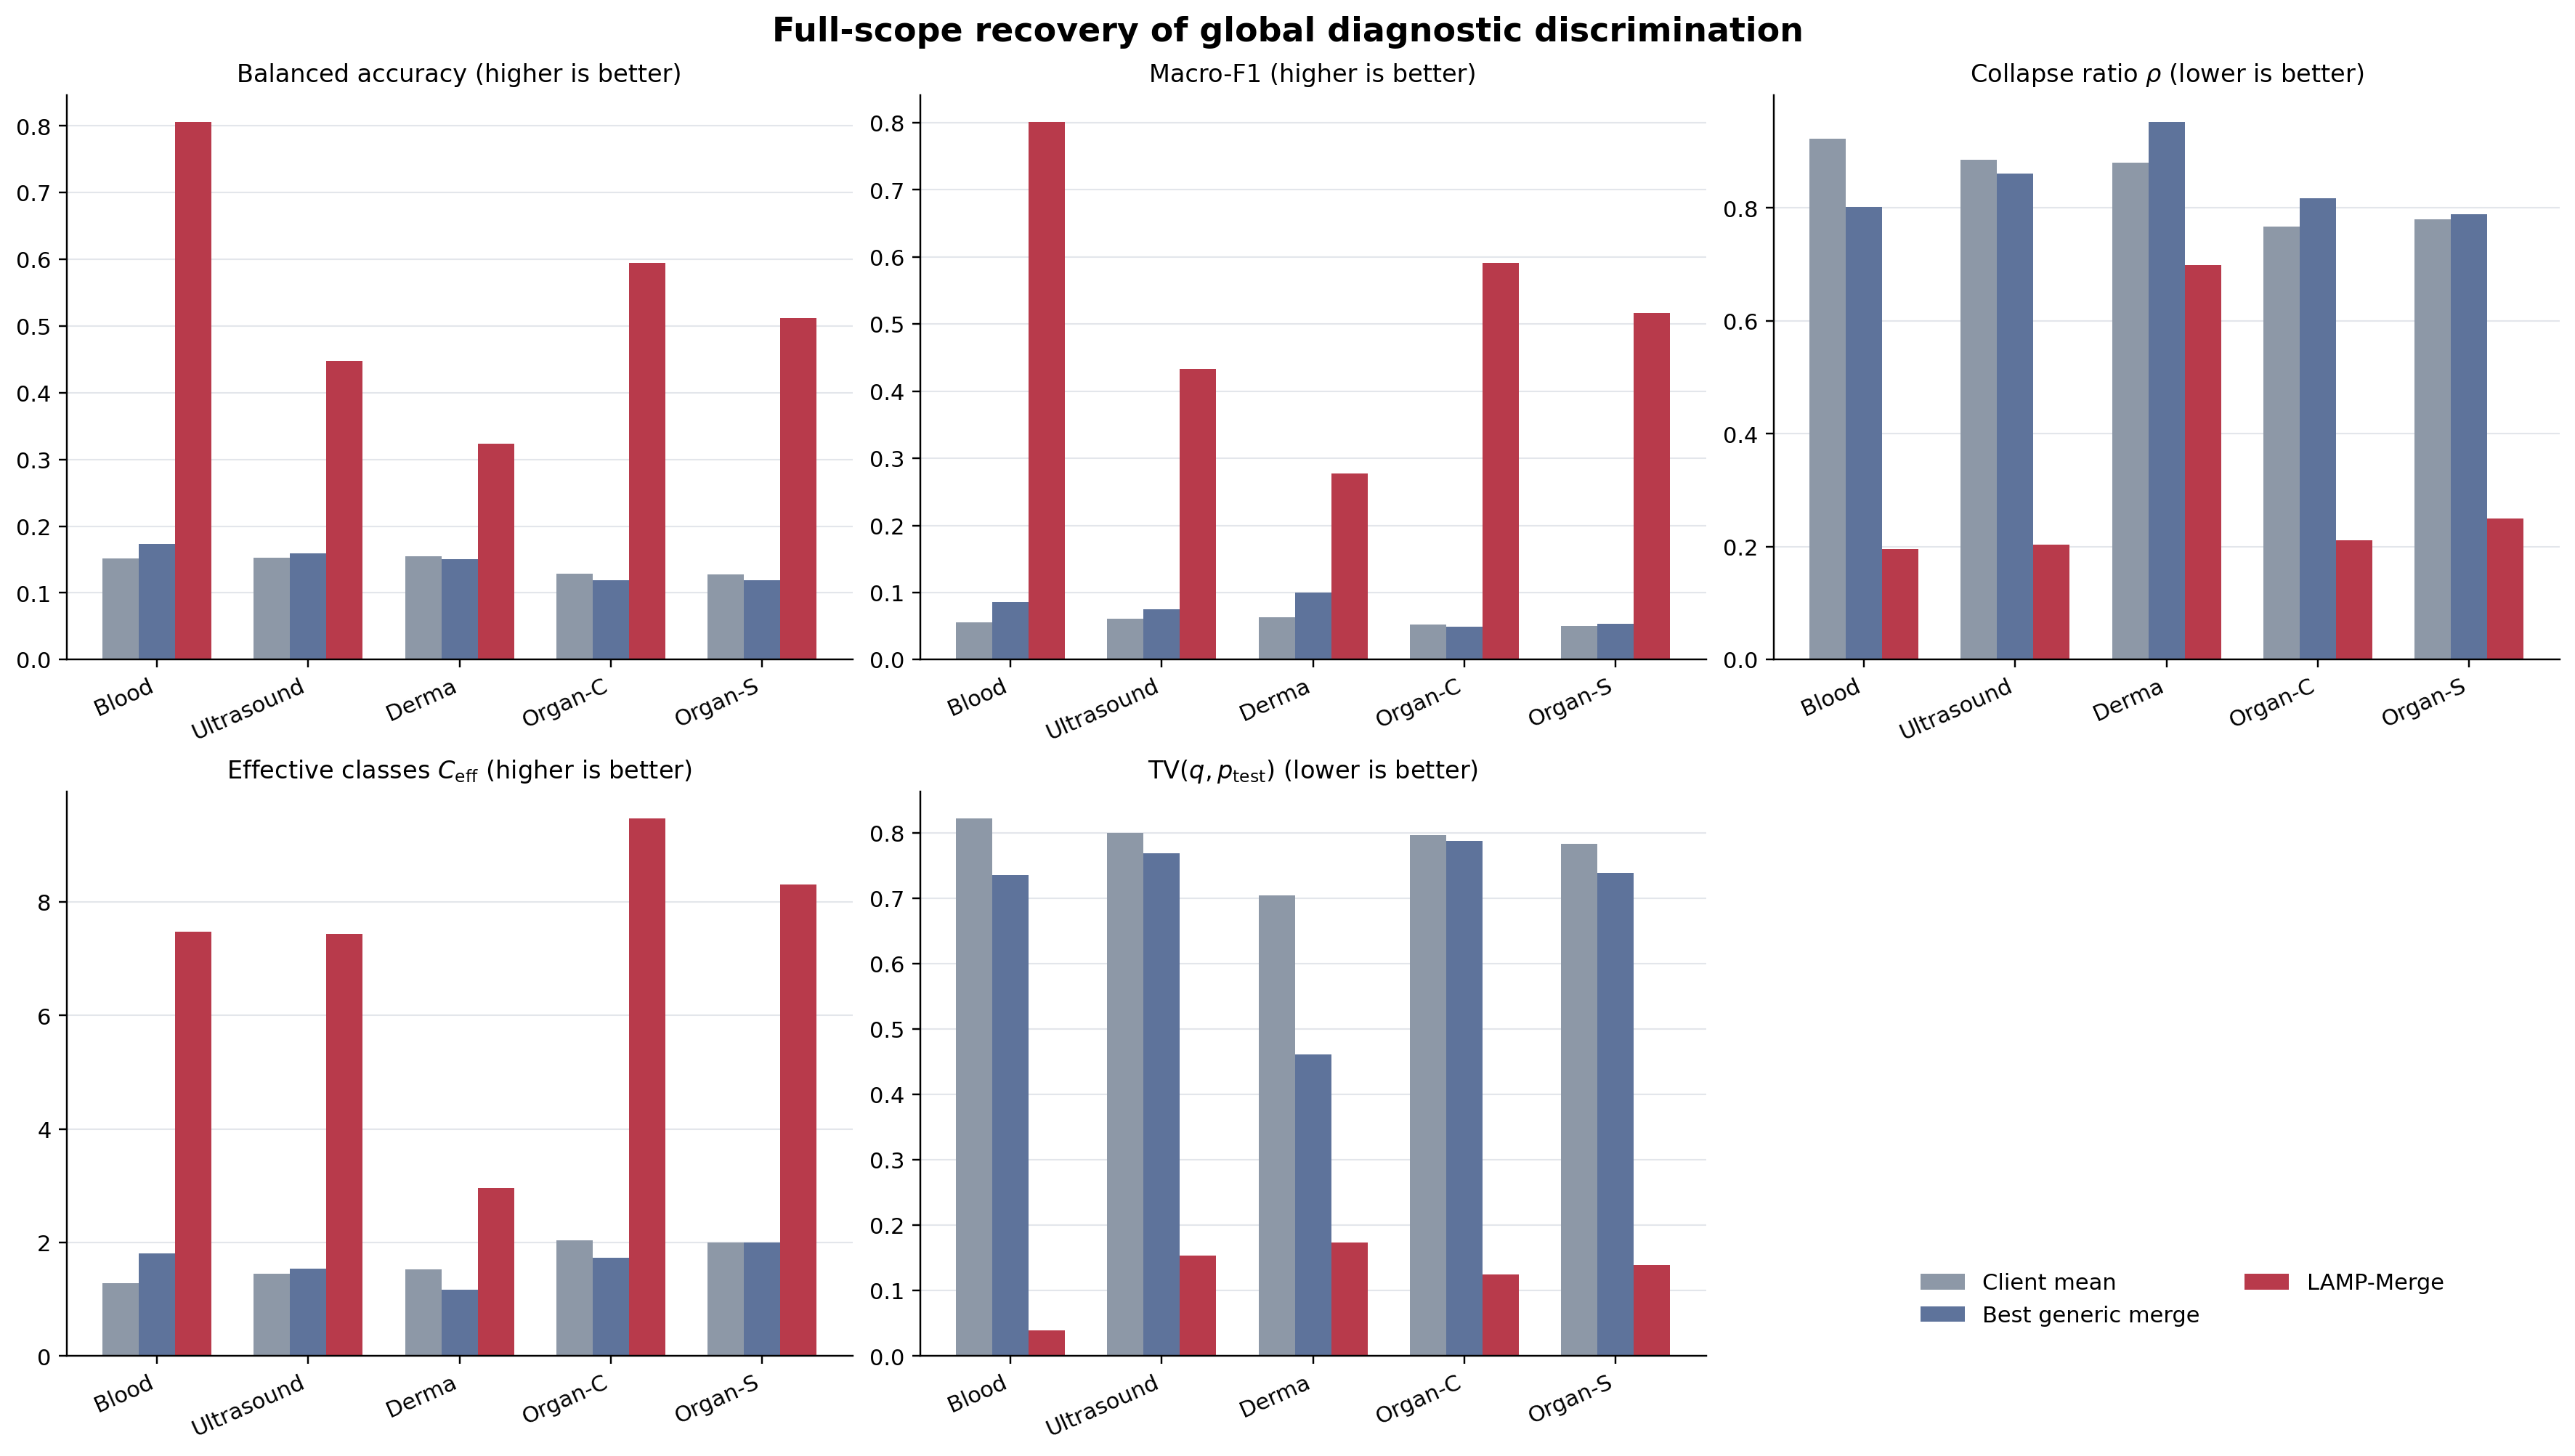
\includegraphics[width=0.94\linewidth]{figures/full_scope_global_diagnostic_discrimination_recovery.png}
\caption{Recovery of global diagnostic discrimination under different datasets.}
\label{fig:collapse-recovery}
\end{figure}

% 表*中将LAMP-Merge与各个指标的最高基线相对比。可以看到，该方法显著优于目前已有的算法。这说明 LAMP-Merge 的准确率提升并非来自更强的单类坍缩，而是来自更完整的全局诊断判别。
Table \ref{tab:collapse-key} compares LAMP-Merge with the best-performing baseline for each metric. LAMP-Merge consistently and substantially outperforms the existing methods. This indicates that its accuracy gains do not arise from more severe single-class prediction collapse, but rather from more complete global diagnostic discrimination.

\subsection{F. Visualization Experiment}

% 为了直观展示新指标诊断所反映的预测分布变化，我们进一步给出预测坍缩恢复图和代表性数据集上的预测类别分布图。
To visually show the prediction-distribution changes measured by the new diagnostic metrics, we further provide a collapse-recovery visualization in figure \ref{fig:collapse-recovery} and a representative predicted-class distribution in figure \ref{fig:visual-chaosheng_predict}. 

\begin{figure}[t]
\centering

\includegraphics[width=0.94\linewidth]{figures/full_scope_predicted_distribution_ultrasound.png}
\caption{Prediction Distribution on the Ultrasound Dataset}
\label{fig:visual-chaosheng_predict}
\end{figure}

\subsection{G. t-SNE Visualization Experiment}
% 所有原型均位于共享参考特征空间 z=phi_0(T(x)) 中。我们仅将 t-SNE 用于分析，而不用于服务器端选择或融合。BLODD 的 LAMP-Merge 原型视图如图所示。
All prototypes live in the shared reference feature space $z=\phi_0(T(x))$. We use t-SNE only for analysis, not for server-side selection or fusion. The joint t-SNE view for Blood and the corresponding LAMP-Merge prototype view are shown in Fig.~\ref{fig:tsne}.

\begin{figure}[t]
\centering
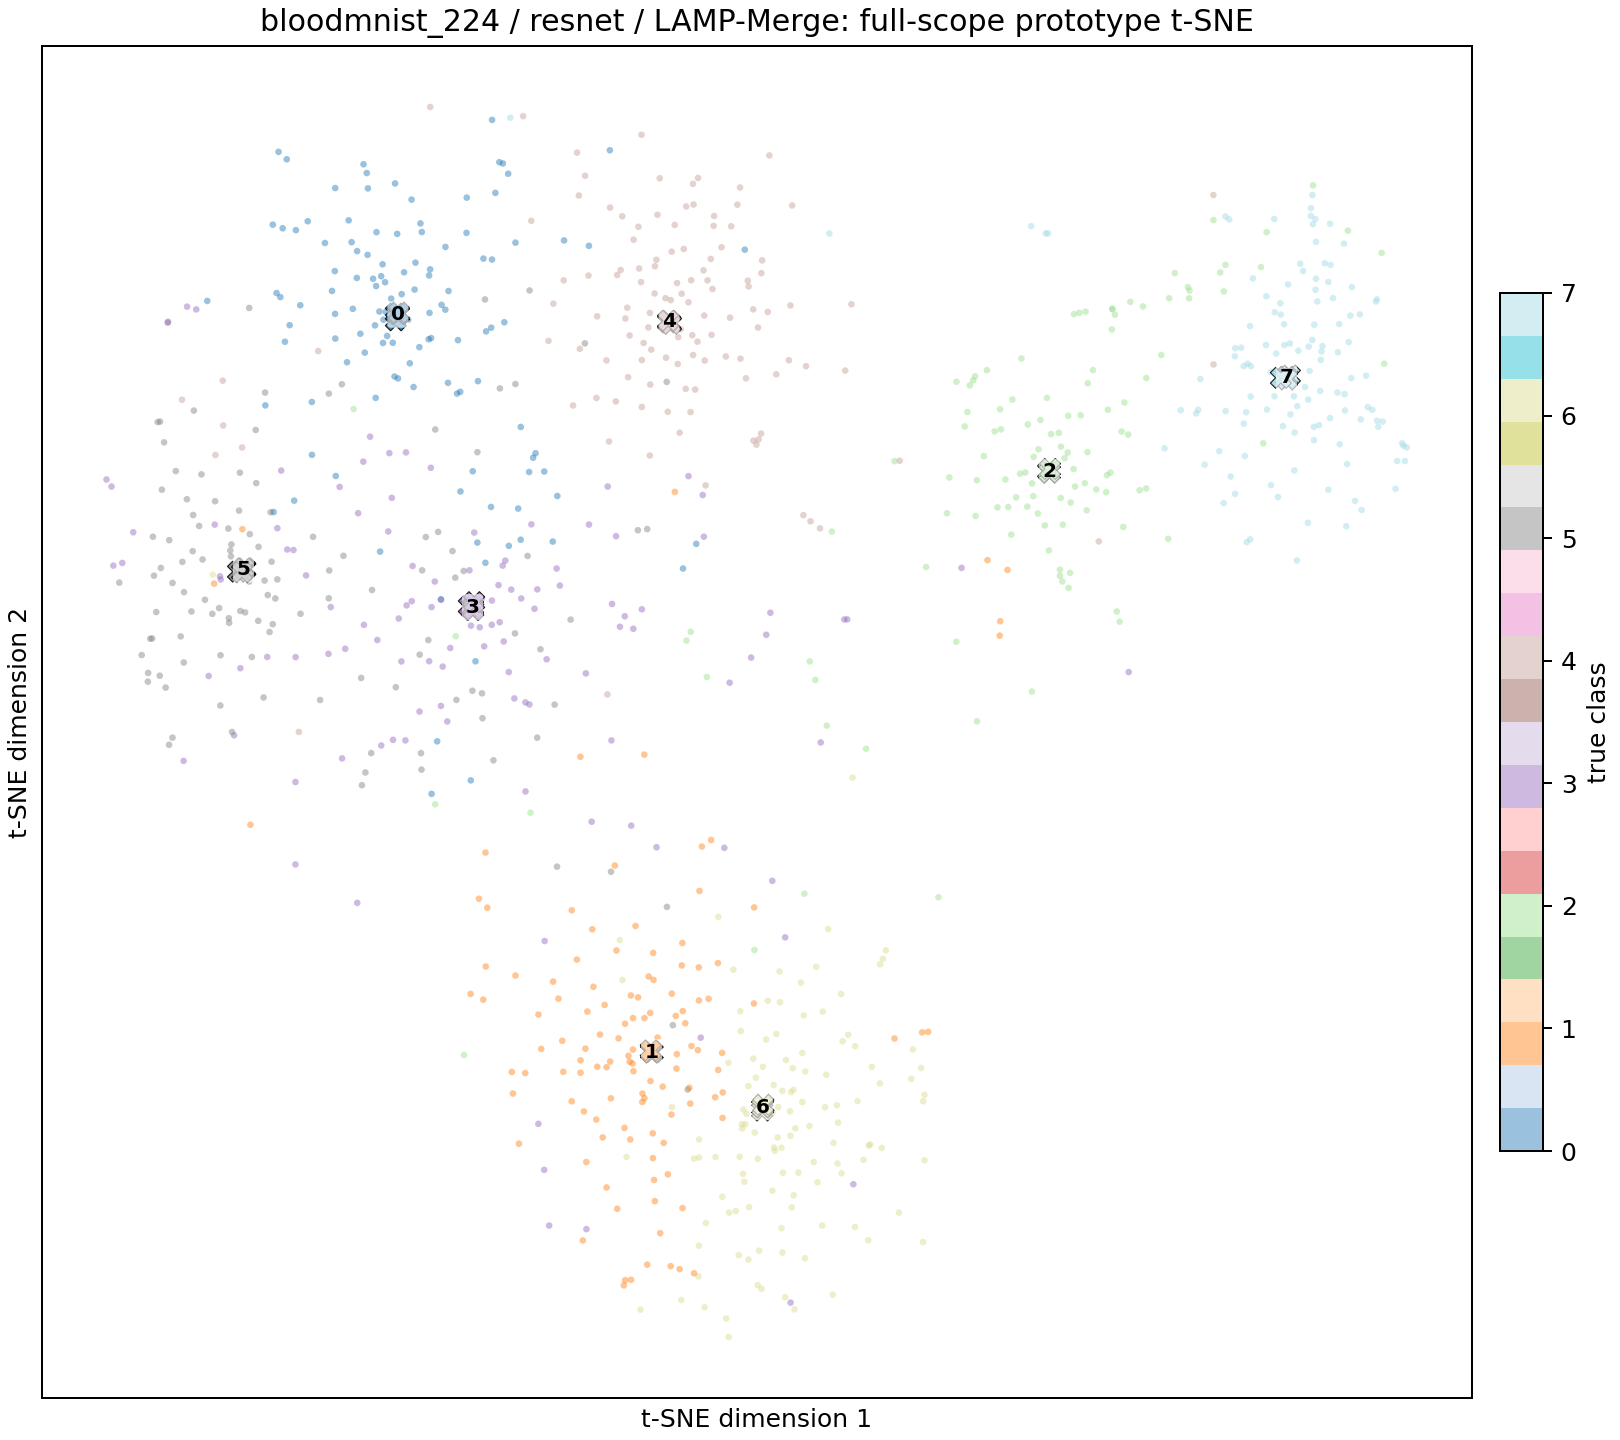
\includegraphics[width=0.82\linewidth]{figures/tsne_lamp_bloodmnist_224_resnet.png}
\caption{t-SNE Visualization of ResNet Feature Representations on the Blood Dataset}
\label{fig:tsne}
\end{figure}

\subsection{H. In-depth Analysis Experiment}
\subsubsection{1) analysis of the geometry}
% 最后，我们对诊断原型重建产生的几何结构进行深入分析。该实验对应模块内消融中的原型替换设置，用于解释为什么共享参考空间类别原型与类别级支持数共同带来稳定收益。令 d(a,b)=1-cos(a,b) 表示余弦距离，令 I_c 表示具有类别 c 样本的客户端集合。所用几何量定义如下。
Finally, we conduct an in-depth analysis of the geometry induced by diagnostic prototype reconstruction. This experiment corresponds to the prototype-replacement settings in the internal ablation and explains why reference-space class prototypes and class-level support counts jointly provide stable gains. Let \(d(a,b)=1-\cos(a,b)\) denote cosine distance, and let \(\mathcal{I}_c=\{i\mid n_{i,c}>0\}\) denote the set of clients that contain diagnosis class \(c\). The geometric quantities are defined as follows.

\begin{itemize}
\item \(D_{\mathrm{pair}}=\frac{2}{C(C-1)}\sum_{c<d}d(p_c,p_d)\). This is the mean distance between global prototypes of different diagnosis classes, measuring whether the reconstructed head forms separable class-level diagnostic directions.
\item \(D_{\mathrm{nn}}=\frac{1}{C}\sum_c \min_{d\ne c} d(p_c,p_d)\). This is the mean nearest-class distance, measuring the most vulnerable decision margin around each diagnosis prototype.
\item \(A_{\mathrm{client}}=\frac{1}{C}\sum_c \mathrm{Avg}_{i<j,\,i,j\in\mathcal{I}_c}\cos(\mu_{i,c},\mu_{j,c})\). This is the within-class consistency among client prototypes, measuring whether clients that observe the same diagnosis produce compatible evidence in the shared reference space.
\item \(A_{\mathrm{proto}}=\frac{1}{C}\sum_c\sum_{i\in\mathcal{I}_c}\alpha_{i,c}\cos(p_c,\mu_{i,c})\). This is the alignment between the server-side global prototype and the contributing client prototypes, measuring whether aggregation preserves client-side class evidence.
\end{itemize}

\begin{figure}[t]
\centering

\includegraphics[width=0.92\linewidth]{figures/full_scope_prototype_geometry_internal_ablation.png}
% 完整基准上的原型几何比较。该图总结了两两距离、最近类别距离、原型一致性和原型-客户端对齐程度。
\caption{Prototype-geometry comparison on the full benchmark. The figure summarizes pairwise distance, nearest-class distance, prototype consistency, and prototype-client alignment.}
\label{fig:prototype-geometry}
\end{figure}

\subsubsection{Additional Theoretical Analysis}
% 令 mu_c^star 表示共享参考空间中的真实类别均值。如果客户端类别特征具有有界二阶矩，则原型估计误差满足如下上界。
Let $\mu_c^\star$ denote the true class mean in the shared reference space. If client class features have bounded second moments, the prototype estimation error satisfies
\begin{equation}
\mathrm{E}\|p_c-\mu_c^\star\|_2^2
\le
\sum_i \alpha_{i,c}^2\frac{\sigma_c^2}{n_{i,c}}
+ \mathrm{Bias}_c^2.
\end{equation}
% 该上界表明，支持数直接控制类别原型估计的方差。没有观测到类别 c 的客户端不应为该类别贡献证据；样本更多的客户端应贡献更多证据，但该贡献应是次线性的。
This upper bound shows that support counts directly control the variance of class-prototype estimation. A client that does not observe class $c$ should not contribute evidence for that class, and a client with more samples should contribute more, but only sublinearly.

% 令样本 x 在类别 c 和 d 之间的真实间隔为 Delta_c,d(x)。
Let the true margin between classes $c$ and $d$ for sample $x$ be
\begin{equation}
\Delta_{c,d}(x)=(\mu_c^\star)^\top z-(\mu_d^\star)^\top z.
\end{equation}
% 当原型误差满足下式时，估计原型能够保持类别 c 和类别 d 之间的排序。
When the prototype error satisfies
\begin{equation}
\|p_c-\mu_c^\star\|_2+\|p_d-\mu_d^\star\|_2
<
\frac{\Delta_{c,d}(x)}{\|z\|_2},
\end{equation}
the estimated prototypes preserve the class order between $c$ and $d$.

% 长尾患病率校准的作用是以有界方式引入长尾先验。对于患病率计数 m_i,c，类别先验为 pi_c，中心化对数先验偏置为 b_c。只要 lambda 有界，长尾患病率校准就不会替代诊断原型重建的判别方向；它只会将输出校准到真实类别患病率。这解释了为什么单独使用长尾患病率校准不充分，而完整 LAMP-Merge 能同时保持非坍缩性和患病率感知能力。
The role of long-tail prevalence calibration is to introduce long-tail priors in a bounded manner. For prevalence counts $m_{i,c}$, the class prior is
\begin{equation}
\pi_c=\frac{\sum_i m_{i,c}}{\sum_k \sum_i m_{i,k}},
\end{equation}
and the centered log-prior bias is
\begin{equation}
b_c=\lambda\left(\log\pi_c-\frac{1}{C}\sum_k\log\pi_k\right).
\end{equation}
As long as $\lambda$ is bounded, long-tail prevalence calibration does not replace the discriminative directions reconstructed by diagnostic prototype reconstruction; it only calibrates the output toward the real class prevalence. This explains why using long-tail prevalence calibration alone is insufficient, while full LAMP-Merge remains both non-collapsed and prevalence-aware.

\section{Conclusion}

% 本文研究了单次异步医学模型融合问题，其中独立训练的医院模型必须在没有联邦优化轮次且不向服务器暴露原始医学图像的条件下被融合。我们的实证分析表明，在局部诊断覆盖不完整时，通用后置融合方法会遭遇聚合诱导的预测坍缩。我们进一步表明，在长尾医学数据集上，这种坍缩可能被原始准确率掩盖，因此设计 Long-tail Prevalence Calibration模块并使用宏召回率、宏 F1 和预测分布诊断进行二次评估。
We studied one-shot asynchronous medical model merging, where independently trained hospital models must be fused without federated optimization rounds and without exposing raw medical images to the server. Our empirical analysis shows that generic post-hoc merging methods suffer from aggregation-induced predictive collapse under incomplete local diagnostic coverage. We further show that, on long-tailed medical datasets, such collapse can be masked by raw accuracy. We therefore introduce the Long-tail Prevalence Calibration module and perform secondary evaluation using macro recall, macro-F1, and predictive-distribution diagnostics.

% LAMP-Merge 以简洁的双模块设计处理这两个性质。未来我们将进一步扩展 LAMP-Merge 的适用范围：一方面，将其从医学图像分类拓展到分割、检测及多模态诊断任务；另一方面，研究更严格的隐私保护机制，例如差分隐私或安全聚合，以进一步降低类别级统计信息可能带来的隐私风险。同时，我们也将探索在更大规模真实多中心医疗场景中的部署与验证。
LAMP-Merge addresses these two properties through a concise two-module design. Future work will extend its applicability in two directions: first, from medical image classification to segmentation, detection, and multimodal diagnostic tasks; and second, toward stronger privacy-preserving mechanisms, such as differential privacy and secure aggregation, to further reduce potential privacy risks associated with class-level statistics. We will also explore deployment and validation in larger-scale real-world multicenter healthcare settings.

\end{document}
